%   *******************************************************************
%   * THIS IS THE MAIN FILE--RUNNING LATEX ON "AllegThesis.tex" WILL  *
%   * GENERATE THE ENTIRE THESIS (ASSUMING YOU HAVE NOT RENAMED IT).  *
%   * IF YOU ARE USING BIBTEX, RUNNING BIBTEX ON "AllegThesis" SHOULD *
%   * GENERATE YOUR BIBLIOGRAPHY. SPECIFIC DETAILS DEPEND ON WHAT     *
%   * ENVIRONMENT AND TOOLS YOU ARE USING (E.G., TEXMAKER OR COMMAND  *
%   * LINE TOOLS LIKE PDFLATEX OR ...).                               *
%   *******************************************************************
%
% AllegThesis.tex
% by A. Thall
% 13 Feb 2003
%
% Revised by R. Roos
% Nov 2013
%
% This document provides a sample Senior Thesis template for use
% by students in Allegheny's CS and Applied Computing programs.
%
%   *******************************************************************
%   * LOOK FOR BLOCK COMMENTS SUCH AS THIS ONE FOR AN EXPLANATION OF  *
%   * THIS DOCUMENT AND HOW TO MODIFY IT FOR YOUR OWN THESIS!         *
%   *                                                                 *
%   * ANY LINE BEGINNING WITH A "%" IS A LATEX COMMENT AND IS IGNORED *
%   * BY THE LATEX PROCESSOR. YOU ARE ENCOURAGED TO COMMENT YOUR OWN  *
%   * LATEX CODE TO HELP YOU REMEMBER WHY YOU DID THINGS A CERTAIN WAY*
%   *******************************************************************
%

%   ********************************************************************
%   * THE FIRST SECTION OF THE MAIN LATEX FILE IS THE "PREAMBLE." IT   *
%   * INSTRUCTS LATEX TO IMPORT SPECIAL PACKAGES FOR THINGS LIKE       *
%   * INCLUDING FIGURES, DOUBLE-SPACING, COLORED TEXT, ETC.            *
%   * DEPENDING ON YOUR NEEDS, YOU MAY FIND IT NECESSARY TO USE PACK-  *
%   * AGES THAT ARE NOT INCLUDED IN THIS TEMPLATE. SIMPLY IMITATE THE  *
%   * "\usepackage{...}" COMMANDS SHOWN BELOW.                         *
%   ********************************************************************

%   ********************************************************************
%   * BEGINNING OF PREAMBLE:                                           *
%   ********************************************************************

\NeedsTeXFormat{LaTeX2e}
\documentclass[12pt]{report}

%   ********************************************************************
%   * ALL BUT ONE OF THE FOLLOWING 5 LINES SHOULD BE COMMENTED OUT.    *
%   * (NOT ALL OF THESE OPTIONS HAVE BEEN TESTED IN THIS REVISION!)    *
%   ********************************************************************

%\usepackage[debug,draft,double]{gatorthesis} % for student proof doublespace
%\usepackage[bottom,double]{gatorthesis} % for final department copy
\usepackage[debug,draft,single]{gatorthesis} % for student workcopy
%\usepackage[single]{gatorthesis} % for student
%\usepackage[debug,draft,nolists,nofront,single]{gatorthesis} % more options


\usepackage{comment}     % provides a way to "comment out" sections in blocks
\usepackage{doublespace} % final document should be double-spaced!
\usepackage{amsmath}     % special symbols
\usepackage{amssymb}     % more special symbols
\usepackage{epsfig}      % needed for including figures
% \usepackage{fancybox}  % --- DISABLED BY RSR, SEP 2013 ---
\usepackage{url}
\usepackage{listings}
\usepackage[figure,linesnumbered,commentsnumbered,lined,boxed]{algorithm2e}
\usepackage{graphicx}
\usepackage{tikz}
\usepackage{subcaption}

%   ********************************************************************
%   * OPTIONAL: IF YOU WANT VERY FINE CONTROL OVER HOW LATEX HYPHENATES*
%   * CERTAIN WORDS, YOU CAN PUT WORDS IN A "\hyphenation" COMMAND AS  *
%   * SHOWN IN THE FOLLOWING EXAMPLE. OTHERWISE, YOU MAY JUST IGNORE   *
%   * THE NEXT COMMAND.                                                *
%   ********************************************************************

% EXAMPLE: Don't hyphenate the words "itself" or "linear". Hyphenate 
%          "representations" only at the places indicated by the "-":

\hyphenation{itself repre-sen-tations linear}

\newcommand{\etal}{\mbox{\emph{et al.\ }}}
\newcommand{\ie}{\mbox{\emph{i. e.\ }}}
\newcommand{\etals}{\mbox{\emph{et al.\ }'s }}

%   ********************************************************************
%   * THE FOLLOWING COMMAND HAS BEEN DISABLED--IGNORE.                 *
%   ********************************************************************
% The following provides a box to surround the thesis statement
%\newenvironment{Thesis}%
%{\begin{Sbox}\begin{minipage}{.95\linewidth}}%
%{\end{minipage}\end{Sbox}\begin{center}\fbox{\TheSbox}\end{center}}

%   ********************************************************************
%   ********************************************************************
%   ***  END OF PREAMBLE.                                            ***
%   ********************************************************************
%   ********************************************************************



%   ********************************************************************
%   * DOCUMENT CONTENT STARTS AT THE "\begin{document}" COMMAND:       *
%   ********************************************************************

\begin{document}

%   ********************************************************************
%   * FILL IN THE "{...}" BELOW WITH YOUR INFORMATION.                 *
%   ********************************************************************

\thesistitle{Intelligent Monte-Carlo Tree Search\\for Perfect Information Games}

\thesisauthor{Lucas Hawk} \thesisadvisor{Dr. Janyl Jumadinova}

\thesisnumber{CS17-05} % SEE PAULINE LANZINE TO GET YOUR REPORT NUMBER!

\thesisreadera{Dr. John Wenskovitch}


%   ********************************************************************
%   * IN RARE CASES YOU MAY HAVE MORE THAN TWO READERS, IN WHICH CASE  *
%   * YOU SHOULD UN-COMMENT THE FOLLOWING AND ADD NAMES:               *
%   ********************************************************************
% \thesisreaderb{Dr. Your Thirdreader} 
% \thesisreaderc{Dr. Your Fourthreader}
% \thesisreaderd{Dr. Your Fifthreader}

%   ********************************************************************
%   * YOU MAY IGNORE THE FOLLOWING COMMAND:                            *
%   ********************************************************************
\date{\FileRevised \\ $\mbox{}$Revision: 1.8 $\mbox{}$}

\thesismaketitle         % Creates the title page
\thesismakecopyright     % Creates the copyright page

%   ********************************************************************
%   * YOU MAY SPLIT YOUR THESIS INTO SEVERAL FILES AND "\include" THEM *
%   * AS SHOWN BELOW. FOR INSTANCE, FILE "abstract.tex" CONTAINS THE   *
%   * ABSTRACT, FILE "ack.tex" CONTAINS THE ACKNOWLEDGMENTS, ETC. YOU  *
%   * MAY, OF COURSE, PUT EVERYTHING INTO ONE HUGE FILE, BUT THERE ARE *
%   * ADVANTAGES TO SPLITTING THINGS UP--FOR EXAMPLE, YOU CAN COMMENT  *
%   * OUT "\include" LINES OF SOME PARTS IN ORDER TO PRINT DRAFTS      *
%   * CONTAINING SELECTED SECTIONS OF YOUR THESIS, SAVING PAPER AND    *
%   * PRINTING COSTS.                                                  *
%   *                                                                  *
%   * YOU ARE NOT REQUIRED TO HAVE A "dedication"--IF YOU DON'T, JUST  *
%   * DELETE THAT LINE OR COMMENT IT OUT WITH A LEADING "%"            *
%   ********************************************************************

\begin{abstract}
Our research focuses on researching areas of research which research has shown to be lacking in research.  Research shows that the research we complete will fill certain gaps in research, making future research easier to research.
\end{abstract}
  % REQUIRED!

%\include{dedication} % OPTIONAL

Thank you caffeine.  You helped more than you know.       % OPTIONAL, BUT ALMOST EVERYONE INCLUDES IT

%   ********************************************************************
%   * FRONT MATTER--TABLE OF CONTENTS, ETC. YOU PROBABLY DON'T NEED TO *
%   * CHANGE ANY OF THIS UNLESS YOU HAVE NO TABLES OR FIGURES, OR YOU  *
%   * WANT TO CHANGE NUMBERING DEPTH FOR SUBSECTIONS, OR ...           *
%   ********************************************************************

\setcounter{tocdepth}{2}    % # of section levels shown in table of contents
\setcounter{secnumdepth}{3} % # of numbered subsection levels in the text

\tableofcontents
%\listoftables       % OMIT THIS IF YOU DON'T HAVE ANY TABLES
\listoffigures      % OMIT THIS IF YOU DON'T HAVE ANY FIGURES

%   ********************************************************************
%   * A GLOSSARY IS ALMOST NEVER NEEDED UNLESS YOU HAVE AN UNUSUALLY   *
%   * LARGE NUMBER OF SPECIAL TERMS OR NOTATIONS AND IT WOULD DETRACT  *
%   * TOO MUCH FROM THE FLOW OF THE PAPER TO DEFINE THEM IN-LINE.      *
%   ********************************************************************
%\include{glossary}  % OMIT THIS IF YOU DON'T HAVE A GLOSSARY (FEW PEOPLE DO)


%   ********************************************************************
%   * THE FOLLOWING "lstset" COMMAND IS ADAPTED FROM ONE FOUND AT:     *
%   * http://tex.stackexchange.com/questions/115467/                   *
%   * listings-highlight-java-annotations                              *
%   *                                                                  *
%   * SEE CHAPTER 3 AND APPENDIX A                                     *
%   ********************************************************************

\lstset{
  basicstyle=\footnotesize\tt, % the size of the fonts that are used for the code
  breakatwhitespace=false,     % automatic breaks only happen at whitespace?
  breaklines=true,             % sets automatic line breaking
  captionpos=b,                % sets the caption-position to bottom
  frame=single,                % adds a frame around the code
  language=Java,               % the language of the code
  keywordstyle=\bf,
  showspaces=false,
  showstringspaces=false,      % underline spaces within strings only?
  showtabs=false,
  tabsize=2                    % sets default tabsize to 2 spaces
}

%   ********************************************************************
%   * NOW INCLUDE THE CHAPTER FILES; COMMENT OUT ANY YOU DON'T WANT TO *
%   * PROCESS IN A PARTICULAR LATEX RUN.                               *
%   *                                                                  *
%   * INCLUDED FILES ARE ASSUMED TO END IN ".tex", E.G.,               *
%   * "ch01_overview.tex", "ch02_relatedwork.tex", ETC.                *
%   ********************************************************************

% ch:intro
%
% $Id: ch01_overview
%
%   *******************************************************************
%   * SEE THE MAIN FILE "AllegThesis.tex" FOR MORE INFORMATION.       *
%   *******************************************************************

\chapter{Introduction}\label{ch:intro} % we can refer to chapter by the label

%   ************************************************************************
%   * In LaTeX, new paragraphs are begun by simply leaving a blank line in *
%   * the LaTeX file.                                                      *
%   *                                                                      *
%   * The \\ characters should NEVER be used to end a paragraph.           *
%   * They are used only for inserting line breaks in certain situations.  *
%   *                                                                      *
%   * "Widows" (ending paragraph lines at the top of a new page) and       *
%   * "orphans" (opening paragraph lines at the bottom of a page) should   *
%   * be eliminated; this sometimes requires re-writing some of the        *
%   * text to change the line lengths.                                     *
%   ************************************************************************

Our research focuses on the development of intelligent agents for playing perfect information games.  Specifically, we implement agents for playing the game Go, Hex, and Sprouts, which we will thoroughly describe later.  The purpose of this chapter is to outline our motivation behind researching this problem, state the goals of our research, and introduce Monte-Carlo Tree Search (MCTS), an algorithm which is very often used for game-playing agents.  We also explain the rules of Go, Hex, and Sprouts, as well as common structures found within the games.

\section{Motivation} \label{sec:motivation}
A major long-term goal of artificial intelligence research is to create a general intelligent agent --- a machine which can act independently, and intelligently, in a variety of situations.  In other words, create a machine which is able to mimic human intelligence.  AI systems already excel in some areas.  For example, in recent years, research into deep neural networks has led to systems which perform very well at pattern recognition problems \cite{imagenet}.  Using a large amount of training data, they are able to perform tasks such as label objects in images\cite{imagenet}, interpret human speech\cite{HintonDeng}, distinguish faces from one another\cite{parkhi15}, and even mimic human speech\cite{wavenet}.  Essentially, such systems can learn to mimic human senses and classification abilities.

However, human intelligence is far more than recognizing patterns and understanding the things we sense.  The ability to react to our world, solve problems, and adapt to changes is much more important when defining true intelligence.  Therefore, in order to progress towards the goal of a more generalized AI, we need to build systems which exist in and adapt to changing environments.

One's first instinct in developing general AI may be to use physical robots as intelligent agents and the real world as an environment.  Robots have been (and continue to be) used in AI research and competitions --- for example, the RoboCup Soccer \cite{robocup} tournament is an annual competition which pits cooperative multi-agent robot systems against one another in games of soccer (Figure \ref{fig:robocup}).  The teams of robots consistently improve every year.  Despite this, their limitations are very obvious.  A quick google search yields many results of the robots failing to do what they were designed to.

\begin{figure}[h]
    \centering
    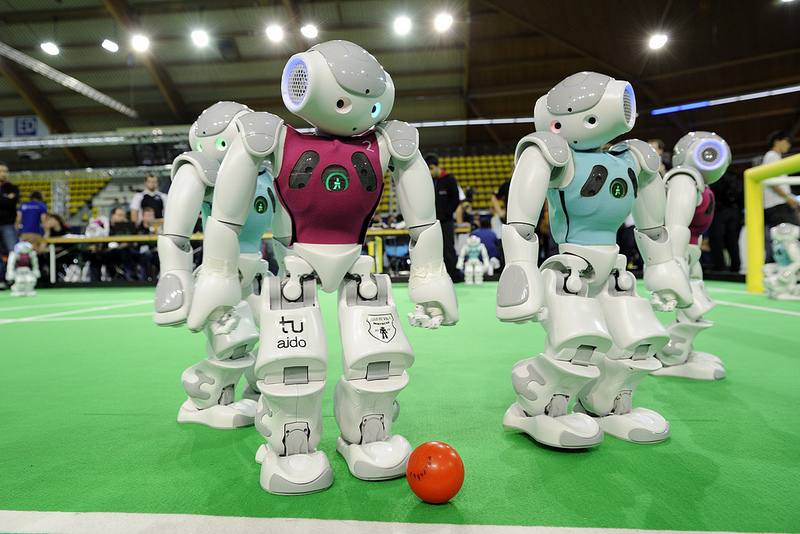
\includegraphics[clip, scale=.25]{images/robocup2015.jpg}
    \caption{RoboCup 2015 \cite{robocup}}
    \label{fig:robocup}
\end{figure}

This is an example of why robots are not ideal for developing AI algorithms --- robots are expensive to build, time-consuming to test, and their effectiveness is bottlenecked by their physical limitations \cite{Gunderson}\cite{Bihlmaier}; they are not an effective way to test algorithms.  Furthermore, there are many variables of the real world which we are simply unable to control effectively, e.g. gravity.  Robots do hold a very important place in the field of AI and computer science in general, but they are not suited for testing new and improving algorithms.  Purely virtual environments --- specifically computer board games --- though, are perfect for experimentation for several reasons.

When working with software agents rather than robots, we do not need to worry about the physical efficacy and limitations of the agents --- the integration of hardware and software is not needed.  Meanwhile, the board game has a set of rules which cannot be broken, and a very obvious goal for everyone in the game: to win.  Furthermore, the rules and win-conditions can be tweaked as needed, and the game can be sped up to allow for quick learning and testing.  Simply put, such games offer extremely controllable environments.  The clear goal (to win) allows for very easy experimentation and testing of game playing agents.  To see how an agent compares against humans, we can simply have the AI play a number of humans to see how often it wins.  We can also have two different agents compete head to head against one another.

Perfect information games are a subset of games for which each player has access to all of the game information --- nothing is hidden from either player.  For example, chess and go are both perfect information board games as both players know the location of any and all pieces on the board.  However most card games, or a game such as Stratego, are imperfect information as the value of each players pieces are hidden from one another \cite{Policonomics}.

When comparing two agents in a head to head game, we consider perfect information to be superior to imperfect information games.  This is because perfect information ensures that the reason for an agent's win is actually a superior algorithm.  In an imperfect information game, there could be pieces of information which are more valuable than other pieces of information --- results of the game could be skewed towards whichever AI stumbles upon this information first \cite{Gilpin}.  For example, in Stratego, the value of a player's piece is hidden from their opponent until an "attack" is made against the piece --- if one player happens to find higher level pieces than their opponent early in the game, the game may become skewed in their favor through pure luck.  While it may be possible to account for such situations (or such imbalances may begin to even out over many trials), it can be easier to just begin with a perfect information game.

In any intelligent game-playing agent, the most important factor is the ability of the agent to evaluate the game state --- that is, the methodology it uses to determine the probability of winning the game for a given state.  For this, one might consider building a system which attempts to identify patterns among positive game states and construct a set of beliefs to approximate the value of any given state; this set of beliefs can be thought of as an evaluation function or heuristic.  However, building an adequate evaluation function for a game state is a very complex task; in fact, there has been much research into using heuristic analysis with little success \cite{chaslot2008monte}.

Tree search methods are another way of determining the value of a game state.  A tree search method simulates a number of full games from the given state, attempting to fully construct a tree of all possible game configurations from the current state --- this tree is called the game tree.  Rather than trying to directly analyze the value of a given game state, a tree search method determines value of a game state by finding how many paths to a winning position exist.

As a tree search algorithm runs, the game tree becomes fuller; once the tree is full, an agent utilizing it is able to play perfectly --- that is it will always win provided it is possible.  The downside of many tree search algorithms is that they are not useful until the game tree is at least mostly full.  In the minimax algorithm, for example, a node's value cannot be determined until the value of every one of its children down to the leaf nodes is found.  For a game such as Go, this is impossible to achieve in any reasonable amount of time --- a single game of traditional 19x19 Go has over $2 \times 10^{170}$ possible playouts.  The exact number of possible Go games was only recently calculated, and required an estimated 30 petabytes of disk I/O \cite{Trompfinal}.  Note this isn't actually constructing the game tree, just calculating how large it would be --- it is actually theoretically impossible to even come close to constructing the whole game tree with today's computing capabilities, due to the sheer amount of storage needed to keep track of everything.

Over the last decade, game AI development has moved away from basic tree search and towards methods involving the Monte-Carlo Tree Search (MCTS) algorithm.  MCTS asymmetrically explores the game tree by taking into account both the current estimated value of each child node, and the number of times each child node has been visited in a simulation.  The specific method of exploration can be customized by considering one of these factors more heavily than the other.  MCTS is also different from other tree search algorithms as it does not need to construct an entire game tree in order to make a decision.  Such methods have proven far more successful, as MCTS-based AIs have since become some of the most successful game AIs in the world \cite{alphago}\cite{benzene}.
%   *******************************************************************
%   * FIGURES ARE PLACED ACCORDING TO A SET OF CONSTRAINTS THAT CAN   *
%   * BE MANIPULATED TO SOME DEGREE.                                  *
%   * A SEARCH FOR "controlling latex floats" TURNS UP A NUMBER OF    *
%   * SITES THAT HAVE USEFUL INFORMATION, FOR EXAMPLE:                *
%   *                                                                 *
%   * http://mintaka.sdsu.edu/GF/bibliog/latex/floats.html            *
%   * http://goo.gl/aC8E8Q                                            *
%   * http://robjhyndman.com/hyndsight/latex-floats/                  *
%   *******************************************************************

\section{Monte-Carlo Tree Search}\label{sec:stateofart}
Monte-Carlo Tree Search (MCTS) is a selective search method for finding optimal decisions via random sampling. Since its development in 2006, it has been widely used for the creation of game AI, specifically for games which can be represented as a finite tree of moves \cite{browne2012survey}\cite{chaslot2008monte}.

MCTS is superior to other popular tree search methods such as minimax for a couple of reasons.  First, while an agent utilizing minimax guarantees optimal play, minimax requires the entire game tree be explored --- this often requires an impractical amount of time for games with even just a moderate branching factor.  MCTS, however, can be interrupted at any time and return a node to explore.  Second, given adequate time, MCTS provides optimal play given adequate memory and time --- in fact, MCTS converges to minimax \cite{browne2012survey}.  So essentially, MCTS can provide accurate decision making without the potentially exponential time complexity of minimax.  

MCTS works in four steps as depicted in Figure 2: Selection; Expansion; Simulation; and Backpropogation.
\begin{enumerate}
    \item  Selection: Starting at the root of the tree, child nodes are selected recursively until a leaf node $L$ is reached.  The way in which these children nodes are selected is called the \textit{tree policy}, and is discussed below.
    
    \item Expansion: if $L$ is not a terminal node for the game tree, a child node $C$ is created.  Depending on the application of MCTS, more than one child node may be chosen.
    
    \item Simulation: Simulate a full play of the game from node $C$.  In the simulation step, the tree policy is not used during the simulation.  Rather, a \textit{default policy} is used --- most commonly, the default policy is a simple random selection from possible moves until a terminal condition is met.  Note that the nodes visited during simulation are not added to the tree.
    
    \item Backpropogation: The tree is updated with the results of the simulation.  Specifically, each node's estimated value is updated (based on the outcome of the simulation), as well as the number of times it has been visited.
\end{enumerate}

\begin{figure}[h]
    \centering
    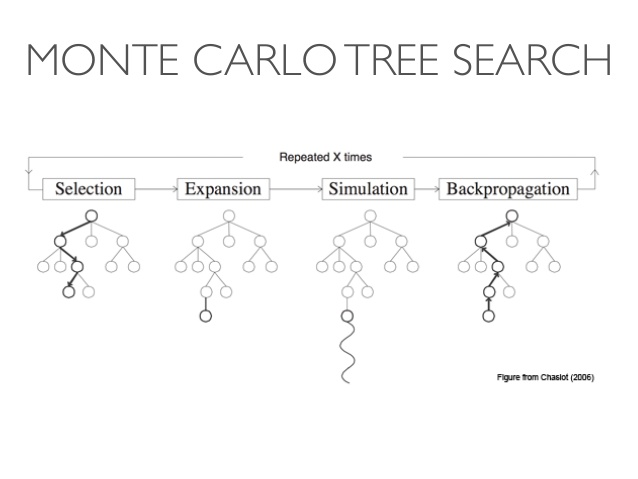
\includegraphics[clip, trim={0 4cm 0 5cm}, scale=.6]{images/mcts.jpg}
    \caption{Monte-Carlo Tree Search algorithm \cite{chaslot2008monte}}
    \label{fig:MCTS}
\end{figure}

During the selection phase, there is a trade-off between \textit{exploitation} and \textit{exploration} --- should we \textit{exploit} the nodes whose rewards we already know, and continue to expand a well searched path, or should we \textit{explore} the less visited nodes in hopes of finding a better option \cite{nakhost2009monte}?  A widely used tree policy to balance these options is called Upper Confidence Bounds for Trees (UCT).  When using UCT as the tree policy, a child node which maximizes the following is chosen:
    
\begin{equation}
    UCT = v_i + C * \sqrt{\frac{2\ln N}{n_i}}
\end{equation}
    
where $v_i$ is the estimated value of the node, $n_i$ is the number of the times the node has been visited and $N$ is the total number of times that its parent has been visited.  $C$ is a constant bias parameter which we can change as we wish.  In this formula, $v_i$ represents exploitation, while the rest of the equation represents exploration.  So, by properly tuning the value of $C$, we are able to find a balance between exploitation and exploration \cite{lucas2014fast}\cite{audibert2009exploration}.

While MCTS can be rather effective in its most basic form, it is further enhanced using a variety of machine learning techniques.  Most of the industry leading game-playing agents utilize an MCTS decision making algorithm with the integration of some other AI techniques --- most often, some form of Artificial Neural Network (ANN) or Genetic Algorithm (GA) is used.  These algorithms and existing implementations of game-playing agents which utilize these algorithms will be discussed in Chapter 2.

%It is the privilege of the thesis author (in consultation with the
%project supervisor and other readers) to decide on the best way to 
%organize the sections and chapters in the way that makes the most sense.
%If the introduction begins with a motivating
%anecdote, perhaps this is best followed by defining a few terms or mentioning
%some major results that the reader should be aware of right from the 
%beginning. But 

\section{Games}\label{sec:goals}
In this brief section, we outline the perfect information games we use for our experiments: Go, Hex, and Sprouts.  Go and Hex are two rather well-known and studied games, while Sprouts has been less popular in research.  The purpose of this short section is to give the reader an understanding of how the games are played.

\subsection{Go}
Go is a two-player game usually played on a 19x19 board, although boards of size 9x9, 13x13, and 17x17 are also common.  The rules of Go are very simple.  The players take turns placing stones on the board, attempting to surround more territory than the other player.  Stones cannot be removed, but if one or more of a player's stones are completely surrounded by the other's, the surrounded stones are removed from the board (Figure \ref{ref:gogui}).  The game continues until either neither player wishes to move or one player resigns.

\begin{figure}[h]
\centering
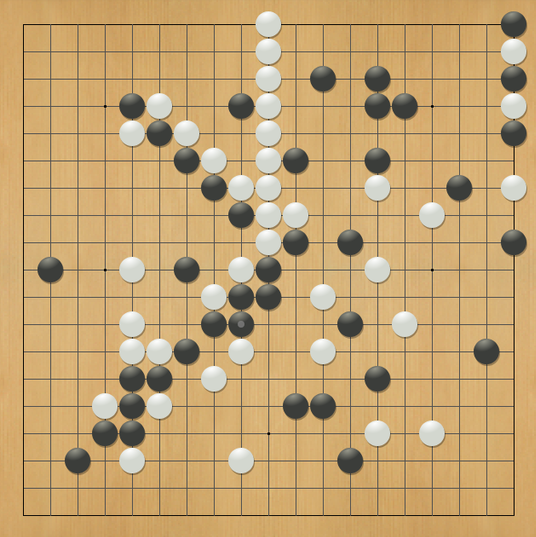
\includegraphics[scale=0.25]{images/gogui.png}
\caption{A Go board generated in GoGui}
\label{ref:gogui}
\end{figure}

Despite its simple rules, Go has over $2 \times 10^{170}$ possible playouts, making it one of the most computationally complex board games ever created \cite{Trompfinal}.  The combination of this fact with its popularity as a game has led to it being the focus of a large amount of research, compared to other games.

\subsection{Hex}
Hex is a two-player board game usually played on a hexagonal grid, usually a 14x14 rhombus as shown in Figure \ref{ref:hex}.  Each player takes turns placing a stone on a cell of the grid, and simply attempts to link their two opposing sides before the opponent links the other two.  The first player to connect their two sides wins.  The only other rule is that, due to the first player to move having a distinct advantage, the second player can choose to switch positions with the first player after the first move.

\begin{figure}[h]
\centering
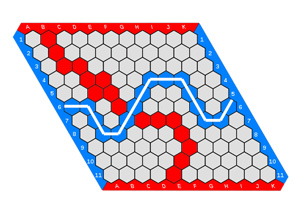
\includegraphics[scale=0.4]{images/hex.jpg}
\caption{A winning game for blue \cite{hexwiki}}
\label{ref:hex}
\end{figure}

\subsection{Sprouts}
Sprouts is a two person pencil-and-paper game which was created by John Conway and Micheal Paterson at Cambridge University in the 1960s. The game has two players, and begins with any number of dots on a piece of paper. The two players take turns drawing a line either between two dots or from one dot to itself. When this line is drawn, a new dot is placed on the line splitting it in half. The last player who is able to legally draw a line wins. A line is only legal if it does not cross any other lines. Furthermore, no vertex can have more than 3 lines coming out of it --- a play on a vertex which already has 3 lines is illegal. The game ends when no moves are possible, and the last player to make a legal move wins.

\begin{figure}[h]
\centering
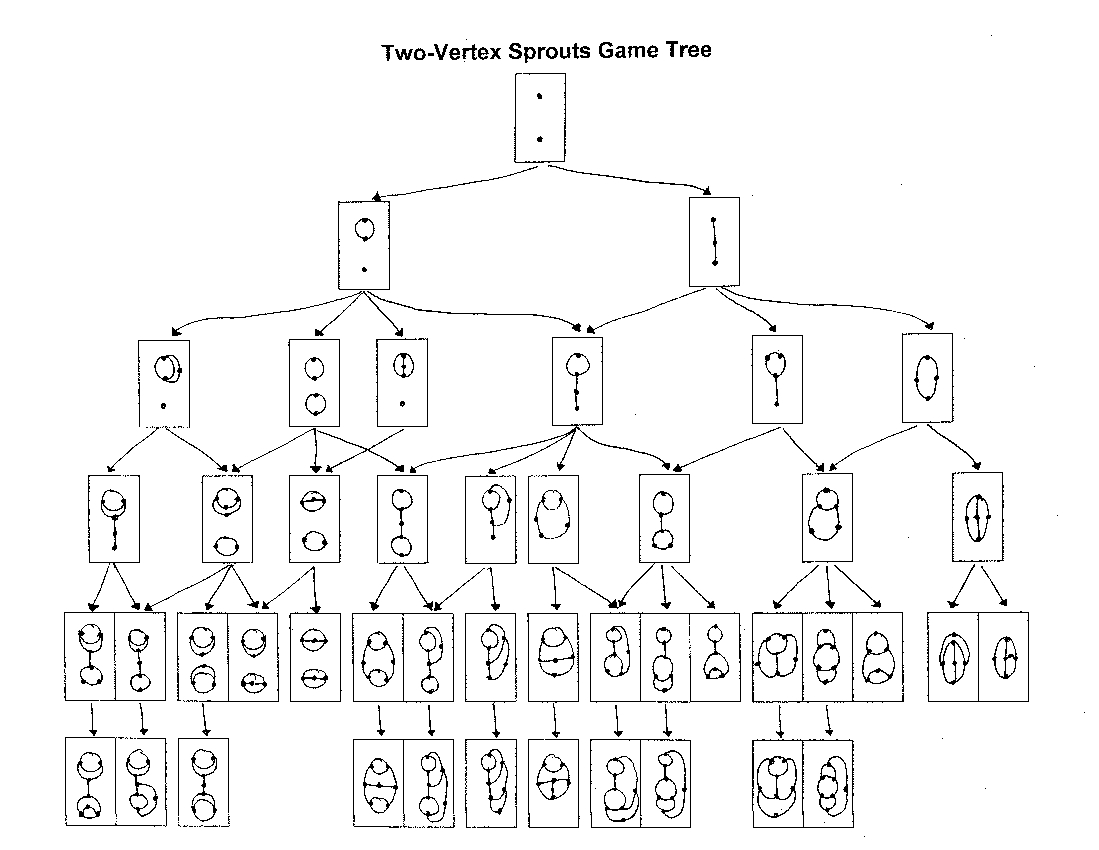
\includegraphics[scale=0.5]{images/sproutsgametree.jpg}
\caption{2 vertex game tree for Sprouts \cite{sproutstree}}
\label{ref:sprouts}
\end{figure}

Figure \ref{ref:sprouts} shows the game tree for the simplest possible game of sprouts --- one with only two starting vertices. As new vertices are added to the start of the game, the tree grows very rapidly.  Because of the simplicity of games with a small number of starting nodes, Sprouts has been completely solved for up to 32 starting vertices --- that is, if the number of starting nodes is at most 32, one can play a perfect game and force a win depending on whether they move first or second \cite{lemoine}.

\section{Goals of the Project}\label{sec:goals}
As stated previously, most of the best current game-playing agents utilize MCTS with some integration of another AI algorithm.  These agents are almost always shown to perform better than agents using just MCTS or other decision making algorithms.  However, they have rarely if ever been directly compared to one another.  This thesis helps fill this gap in research.  We implement a number of intelligent game-playing agents using MCTS integrated with machine learning algorithms which have been utilized in current, leading systems. These agents are benchmarked against one another on several perfect information games: Sprouts, Go, and Hex.  This provides a concrete, direct comparison of existing techniques, and a clear heirarchy between these techniques is shown.

The use of multiple games is important in these tests.  While the performance of standard MCTS is game-independent, the performance of heuristic techniques is often quite dependent on the game, as stated earlier.  When we integrate MCTS with these different AI algorithms, we are essentially introducing a small heuristic bias in the way MCTS performs.  Using multiple games helps show how this introduction of a heuristic bias affects how game-dependent the performance of the agent is.

% COMMENTED OUT NEXT FEW LINES TO SAVE SPACE; MAY PUT THEM BACK LATER
%Following the concise statement of the thesis, some of the details can be
%expanded.  
%It is appropriate to
%refer to some of the results in the introduction (which may 
%mean going back and adding them to the introduction once the
%research is completed). 
%A senior thesis, or any research paper, is not a mystery 
%novel---there is no need to keep the reader in suspense about what
%has been accomplished.

\section{Thesis Outline}\label{sec:outline}
Chapter two introduces the different AI algorithms we integrate with MCTS, and also describes current implementations utilizing these algorithms.  Each section of the chapter focuses on a different algorithm, and outlines a game-playing agent which has been implemented using such an algorithm.  Chapter three goes over our experiment design, testing methods, and any possible validity concerns are also discussed.  In Chapter four, we overview Fuego, the library we use to implement our agents, as well as the actual design of each agent.  Finally, we discuss our results and future research in Chapter five. % Introduction -- of course, you can name it anything!

% ch:relatedwork
%
% $Id: ch02_relatedwork
%
%   *******************************************************************
%   * SEE THE MAIN FILE "AllegThesis.tex" FOR MORE INFORMATION.       *
%   *******************************************************************
\chapter{Related Work}\label{ch:relatedwork}
In this chapter, we discuss the different algorithms we integrate into MCTS, as well as describe existing implementations of game-playing agents which use these techniques.  In addition to explaining the algorithms we are using, we also describe the algorithm behind Google's AlphaGo, the current world-champion computer Go agent.  The chapter is organized by algorithm, with each section discussing a specific algorithm and existing implementation of the algorithm.  We discuss how each existing system has been implemented, and briefly overview how well these implementations have performed.  After this, we describe the Encog machine learning library which is used in our implementation.

\section{Genetic Algorithms}
A Genetic Algorithm (GA) is an optimization or search algorithm based on Darwin's theory of evolution \cite{fuzzymitchell99}.  The algorithm borrows ideas from biology such as genes and chromosomes, as well as the concepts of crossover and mutation.  In biology, a gene can be thought of an encoding of a trait, such as eye color, while a chromosome is a collection of genes which make up the ``blueprint" of an organism.  Crossover is the process of selecting genes from two parent chromosomes to create a child chromosome, while mutation is a random alteration of a gene.  Before explaining how a GA works, it is important to first understand what these terms, and a few others, mean in regards to the algorithm.

In GAs, a chromosome refers to a possible solution to a problem, which is often encoded as a string of bits.  The genes are the various chunks of the chromosome which encode a specific element of the solution.  For example, consider an agent from a GA which trades on the stock market.  Every stock indicator (such as change in price, volume, etc.) may be represented by a gene consisting of 4 bits --- the value of each gene determines how highly it considers that indicator compared to the others.  The agent's chromosome is made up of a collection of these genes and is its overall trading strategy.  Crossover might consist of randomly selecting genes from two agents to create a new chromosome, while mutation might be	having a possibility of flipping a random bit in a gene.

Furthermore, the entire collection of chromosomes (i.e. potential solutions) is referred to as the \textit{population}.  The \textit{fitness} of a particular chromosome is essentially how good of a solution it provides; the \textit{fitness formula} $f(x)$ is the method of calculating fitness.  On each iteration of the algorithm, a new population is created --- each population is referred to as a \textit{generation}.

A GA begins by generating a random population for the problem space.  Then, the fitness of each member of the population is calculated by some $f(x)$; a chromosome's fitness may also just be an amount relative to the fitness of other chromosomes.  Next, we repeat the following steps until $n$ new chromosomes have been created:
\begin{itemize}
\item Select a pair of chromosomes (parents) from the population.  The probability of selection is higher for chromosomes with a higher fitness;
\item Via some predetermined method, perform a crossover between the two parents to create a child chromosome;
\item Randomly mutate the child chromosome with a predetermined probability $p_m$.
\end{itemize}

Once $n$ children have been created, we replace the $n$ lowest performing children in the population with the new children --- this creates our new generation.  This process of evaluation, selection, crossover, and mutation repeats itself until either (a) a desired fitness is reached or (b) a certain number of generations has been produced.  Figure \ref{fig:GA} depicts the GA algorithm visually; each box in the figure represents a different member of the population, while the different colors represents different ``genetic makeups'' of each chromosome.

Note that the crossover portion of the algorithm helps improve the overall fitness of the population over time, while the mutation helps maintain diversity in the population and protect from the chromosomes becoming overfit.  These concepts, as well as the random distribution of chromosomes over the search space  at the start, help keep the algorithm from getting stuck at local maxima.

\begin{figure}[h]
    \centering
    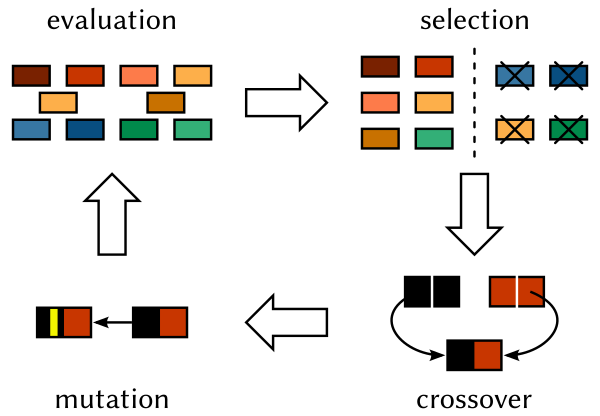
\includegraphics[clip, scale=.3]{images/GA1.png}
    \caption{Process of a Genetic Algorithm}
    \label{fig:GA}
\end{figure}

A GA can be integrated with MCTS to fine-tune both the tree policy and the default policy.  In \cite{Cazenave2007}, Cazenave created a Go-playing agent which utilized MCTS whose UCT exploration parameter was optimized by a genetic algorithm.  He compared three agents: one whose tree policy was a static UCT, one which used a tree policy known as RAVE \cite{rave}, and finally one with UCT whose exploration parameter he optimized with a GA.  The agent with the optimized bias parameter consistently outperformed the other two.

More interesting is Lucas \etals fast evolution method \cite{lucas2014fast}.  Rather than pre-optimize the MCTS algorithm, Lucas \etal developed a system which optimizes its performance on the fly.  Rather than evaluate individuals after entire game playouts, each iteration of the MCTS algorithm is followed by the evaluation of a number of individuals all working on the same search tree.  At every iteration, both the tree policy and the default policy is biased towards the most fit individuals policy.  The results of Lucas \etals work were positive, showing their algorithm performed better than a standard MCTS agent in 99\% of runs in games called \textit{Space Invaders} and \textit{Mountain Car}.

\section{Artificial Neural Networks}
An Artificial Neural Network (ANN) is a machine learning method which, like genetic algorithms, has a basis in biology --- it is often viewed as a simplified model of how the brain solves problems \cite{aimodern}.  ANNs  are commonly used for pattern recognition or data classification.  Very abstractly speaking, an ANN is simply a cluster of nodes connected by links, with each link having a numerical weight associated with it.

More specifically, each node takes in a number of inputs and produces a decimal output (usually a number between 0 and 1).  Some nodes are connected to the network's environment and are called \textit{input nodes} or \textit{output nodes}.  As one might imagine, input nodes are those which receive data or information from the environment, and output nodes give us the a value based on the network's inputs.  Any other nodes in the network are called \textit{hidden nodes} because they cannot be directly observed/accessed from the environment --- their inputs are either the output of input nodes or other hidden nodes.

Each link between the nodes has a weight associated with it, which essentially just tells each node how much to ``value'' a given input.  There are a few ways in which the nodes and links of an ANN can be structured, and each type of structure (or \textit{topology}) results in different computational properties.  Here, we will specifically talk about \textit{feed-forward} networks as this is the structure we will be using in our experiments.  The other main type of network is the \textit{recurrent} ANN, and often has a more complex topology.

In a feed-forward network, links are unidirectional and there are no cycles --- a feed-forward network is a directed acyclic graph.  The network is organized in layers, with each node only linking to nodes in the next layer.  Although this structure is much simpler than that of a recurrent network, feed-forward networks have sufficient computational abilities for most pattern recognition and classification problems \cite{pruningsource7}.  A simple illustration of a feed-forward ANN with one hidden layer can be seen in Figure \ref{ref:simpleann}.

\begin{figure}[h]
\centering
\def\layersep{2.5cm}

\begin{tikzpicture}[shorten >=1pt,->,draw=black!50, node distance=\layersep]
    \tikzstyle{every pin edge}=[<-,shorten <=1pt]
    \tikzstyle{neuron}=[circle,fill=black!25,minimum size=17pt,inner sep=0pt]
    \tikzstyle{input neuron}=[neuron, fill=black];
    \tikzstyle{output neuron}=[neuron, fill=black];
    \tikzstyle{hidden neuron}=[neuron, fill=black];
    \tikzstyle{annot} = [text width=4em, text centered]

    % Draw the input layer nodes
    \foreach \name / \y in {1,...,4}
    % This is the same as writing \foreach \name / \y in {1/1,2/2,3/3,4/4}
        \node[input neuron, pin=left:Input \#\y] (I-\name) at (0,-\y) {};

    % Draw the hidden layer nodes
    \foreach \name / \y in {1,...,5}
        \path[yshift=0.5cm]
            node[hidden neuron] (H-\name) at (\layersep,-\y cm) {};

    % Draw the output layer node
    \node[output neuron,pin={[pin edge={->}]right:Output}, right of=H-3] (O) {};

    % Connect every node in the input layer with every node in the
    % hidden layer.
    \foreach \source in {1,...,4}
        \foreach \dest in {1,...,5}
            \path (I-\source) edge (H-\dest);

    % Connect every node in the hidden layer with the output layer
    \foreach \source in {1,...,5}
        \path (H-\source) edge (O);

    % Annotate the layers
    \node[annot,above of=H-1, node distance=1cm] (hl) {Hidden layer};
    \node[annot,left of=hl] {Input layer};
    \node[annot,right of=hl] {Output layer};
\end{tikzpicture}
\caption{A simple feed forward ANN}
\label{ref:simpleann}
\end{figure}

With this network structure, learning is just the process of tuning the weights of the links to better fit the data in a training set.  For example, suppose we have a network which we are training to identify handwritten numbers.  If, during training, it identifies a number as a `2' when it is really a `3', it can make a very small adjustment in its weights to get a little closer to thinking it is a `3'.  Over a large data set, these small adjustments add up to create a rather well-generalized network.  Statistically speaking, the ANN is an abstracted, finely tuneable nonlinear regression of the training data \cite{aimodern}. 

In \cite{annpruning}, Burger \etal provide a method of integrating a feed-forward ANN with MCTS --- specifically, they integrate the ANN into the UCT tree policy.  The ANN is used to \textit{prune} the search tree as the agent searches.  That is, it determines that certain portions of the tree are undesirable and removes them from the search space.  Assuming this is done accurately, the tree policy becomes more efficient as it does not spend time expanding the tree in an undesirable area.  A number of pruning schemes are tested, and they determined that exponentially decreasing how much of the tree is pruned as the game goes on performs best.  Burger \etal did not directly test their pruning algorithm against any other agents --- their research only showed that an agent with an exponentially decaying pruning policy outperformed agents with other pruning policies.  

\section{Neuroevolution}
Neuroevolution is a type of machine learning algorithm which uses genetic algorithms to train and evolve neural networks.  In its most basic form, neuroevolution uses evolutionary methods to fine-tune the weights of an ANN whose topology has already been established \cite{aimodern}.  This, of course, will improve the performance of a given ANN over time.  However, the weights of the links between nodes are not the only thing affecting the performance of the network --- just as important, if not moreso, is the actual structure of the ANN \cite{NEAT}.

In \cite{NEAT}, Stanley and Miikkulainen introduce a neuroevolution method called \textit{Neural Networks through Augmenting Topology} (NEAT).  As its name would imply, NEAT is a method of augmenting the topology of neural networks using evolutionary methods.  In NEAT, a population of neural networks is evolved throughout the training process to improve its classification abilities.  Rather than only tune the weights of a network, NEAT trains the network by also changing the structure of the network.

Prior to the evolutionary training process, the number of input and output neurons are defined --- the input and output layers are not changed during training.  The type of activation function to be used is also defined.  No other structure is given to the network, and a population of networks are generated, each with a random structure of hidden neurons, neuron links, and weights.  During training, the worst performing networks are replaced with children of the best performing networks periodically, until an appropriately performing network is found.  A more in-depth explanation of the methodology behind this technique is described in \cite{NEAT}.

Hypercube-based NEAT (HyperNEAT) is an extension of NEAT.  The HyperNEAT extension is uses a similar technique as NEAT, but is specifically meant to be used on very large scale neural networks.  HyperNEAT trains and evolves neural networks to recognize patterns in data such as repetition or symmetry using by using \textit{Compositional Pattern Producing Networks} rather than standard ANNs.  The most unique and novel aspect of HyperNEAT is its ability to create networks which understand the geometry of the problem. \cite{HyperNEAT}

When a normal ANN is used to represent a game board such as Go, it has no concept of the nodes representing spaces set up in a grid; it doesn't actually know where pieces physically are in relation to one another without figuring it out on its own.  HyperNEAT, though, utilizes what is called a \textit{substrate layer} to provide the input and output layer with a representation of the board's geometry.  HyperNEAT creates network connections based on this physical board geometry.  HyperNEAT evolves the network connections over time with a particular board structure already understood prior to training.  Since there are hypothetically several ways to represent the geometry of the game board for any given game, there are several different ways to train a network with HyperNEAT.  For a further explanation of HyperNEAT and an analysis of the algorithm's performance, see \cite{HyperNEAT}.

Figure \ref{fig:neatnet} shows a neural network for an arbitrary problem at two different stages in HyperNEAT --- generation 30 of the network is shown on the left, and generation 106 of the network is shown on the right.  The figure shows how a grid-like structure is given to the network.  Note the differences in connection weight, number of hidden neurons, and overall network structure between the two generations of the network.

\begin{figure}[h]
\centering
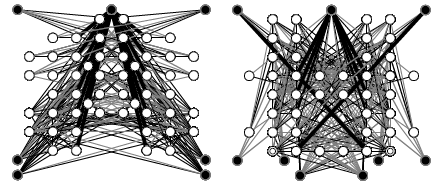
\includegraphics[scale=0.55]{images/hyperneatnets.png}
\caption{A network at two different stages in HyperNEAT \cite{hyperpic}}
\label{fig:neatnet}
\end{figure}

Gauci and Stanley demonstrate how both NEAT and HyperNEAT can be used for Go in \cite{hyperneatgo}.  They demonstrate that an agent utilizing HyperNEAT is able to intelligently play Go, and more importantly, it is able to scale to larger board sizes after only being evolved on a 5x5 board.  While they do not use MCTS in their implementation, they do state that it is very possible to bootstrap MCTS with a tree policy evolved by NEAT or HyperNEAT.  Specifically, they state these algorithms could be used to evolve a more effective default policy for UCT.  This is precisely what we do in our implementation.

\section{Deep Convolutional Networks and AlphaGo}
Deep Convolutional Networks (DCNs) are another class of machine learning algorithms closely related to ANNs.  DCNs are a subset of feed-forward ANNs which contain a number of what are called \textit{convolutional} hidden layers, and are traditionally created for image recognition.  However, as seen in Google's Go playing machine AlphaGo \cite{alphago}, DCNs can be adapted for other tasks as well.

DCNs are far more complex than a simple feed-forward ANN, and to understand them it is perhaps best to think of each layer as a square of nodes rather than a line (Figure \ref{ref:dcn1}).  Each layer still only directly interacts with the very next layer, but each hidden node will only be connected to a small region or window of the input nodes.  This window then ``slides'' over the input layer for each hidden node, with overlap.  This concept is awkward to explain in words, but Figure \ref{ref:dcnmain} represents how this works graphically.

\begin{figure}[h]
\centering
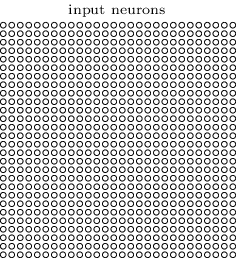
\includegraphics[scale=0.5]{images/dcn1.png}
\caption{DCN input layer \cite{handwriting}}
\label{ref:dcn1}
\end{figure}

This mapping of small windows of nodes onto a single node through several hidden layers is repeated over a number of layers.  After the convolutional layers, there are a series of \textit{pooling} or \textit{subsampling} layers.  These are similar to the convolutional layers in that they still link a region of nodes onto a node in the next layer, but in much smaller groups, perhaps 2x2.  The output of each pooling layer is usually either the maximum or the minimum value from its grid of inputs.  The goal of this process is to simplify the output of the convolutional layers.

\begin{figure*}[h!]
    \centering
    \begin{subfigure}[t]{0.5\textwidth}
        \centering
        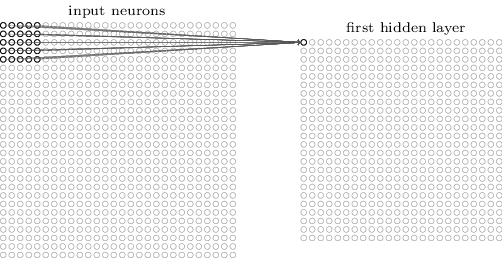
\includegraphics[height=1.4in]{images/dcnmain1.png}
        \caption{Links from input layer to hidden node 1}
    \end{subfigure}%
    ~ 
    \begin{subfigure}[t]{0.5\textwidth}
        \centering
        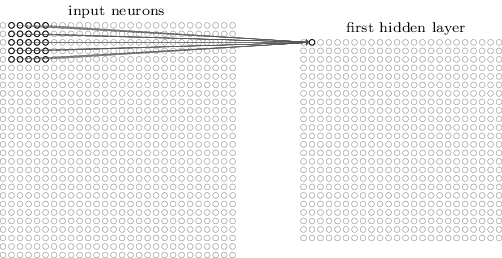
\includegraphics[height=1.4in]{images/dcnmain2.png}
        \caption{Links from input layer to hidden node 2}
    \end{subfigure}
    \caption{Links in a convolutional network\cite{handwriting}}
    \label{ref:dcnmain}
\end{figure*}

The pooling layers are linked with another layer of convolutional layers in the same way convolution was described before, and this back-and-forth between pooling and convolution is done how ever many times is wanted.  This process as a whole is called \textit{feature extraction}, because it allows the network to break a picture down into a representation of its most basic features.  After feature extraction, the final layers are connected to a standard, fully connected ANN which produces the output, usually a classification of the image.

\begin{figure}[h]
\centering
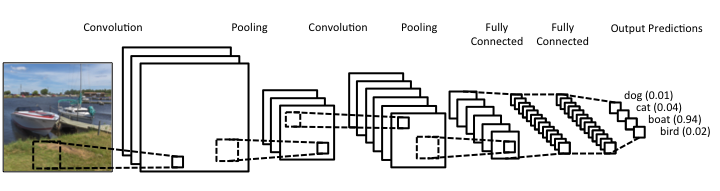
\includegraphics[scale=0.5]{images/cnnfull.png}
\caption{An example of a full DCN \cite{clarifai}}
\label{ref:cnnfull}
\end{figure}

Perhaps the most famous implementation of a DCN with MCTS is Google DeepMind's Alphago \cite{alphago}.  AlphaGo is designed by Google DeepMind which plays the board game Go, and in 2015, it became the first computer program to beat a professional human Go player without handicaps on a full board.  AlphaGo uses MCTS in conjunction with three different DCNs --- two are called ``policy networks'' and essentially alter the tree and default policy of MCTS, while the third is a ``value network'' and helps determine the value of the current game state.  Each network had 13 hidden layers.

AlphaGo was trained in two phases. First, the network was trained on millions of moves from professional Go games. This training was done until the program could predict a human move 57\% of the time. The second phase of training involved AlphaGo playing itself and, using reinforcement learning, discovering new strategies for itself. The result was an incredibly intelligent system --- AlphaGo was able to beat the next best Go AIs in 499 out of 500 games played, even when giving the other programs a four move headstart.\cite{alphago}

Unfortunately, creating an agent as sophisticated as AlphaGo was simply not feasible given our timeframe and resources.  Training a deep convolutional neural network requires training sets which are many magnitudes larger than what is necessary for more simple ANNs.  While Google has the resources necessary to provision such large datasets, we do not.  Furthermore, assuming we did have access to an appropriate amount of training data, training a DCN with 13 hidden layers would require a massive amount of processing power and would be a long, arduous process.

\section{Encog Machine Learning Library}
To ease the integration of each machine learning algorithm into MCTS, we utilized Heaton Research's Encog machine learning library for Java \cite{encog}.  The library has been in active development since 2008, and has been used in a variety of other well-cited research publications since its release (e.g. \cite{encogref1, encogref2, encogref3}).  We chose this library because of its wide use, thorough documentation, and large number of example programs provided.

Encog provides functionality for most common machine learning algorithms, including genetic algorithms, artificial neural networks, and NEAT/HyperNEAT.  Creating and training these structures is quite easy.  For example, to create and train a simple ANN, you simply create a \texttt{BasicNetwork} object, define the network's structure, create a training dataset, and run \texttt{ResilientPropogation.iteration} on the network and training data to perform a training epoch.  Implementing other machine learning algorithms is just as simple. % Background, literature survey, ...

% ch:method
%
% $Id: ch03_thework.tex
%
%   *******************************************************************
%   * SEE THE MAIN FILE "AllegThesis.tex" FOR MORE INFORMATION.       *
%   *******************************************************************
%
\chapter{Implementation} \label{ch:method}
This chapter provides an overview of the implementation of the Go and Hex classes, the game-playing agents, and the games framework.  Furthermore, we outline our experiments and the methods of running these experiments; the results of the experiments will be discussed in the next chapter.  In each section, we provide both high-level descriptions of the relevant code structure as well as in-depth, low-level discussion of any important algorithms.  The chapter is organized such that the entire code structure is explained from the inside out.  That is, we first describe the games, then the agents which play the games, and finally the framework which orchestrates the playing of the games.  This is because an understanding of each of these parts of the implementation is beneficial to understanding the following parts.

Before the discussion of the more involved classes, we need to first explain the \texttt{Board.java} class, a very simple object which is used in almost every other class.  The \texttt{Board} object provides a representation of a game-independent game board --- there is no game-specific functionality in a \texttt{Board} object.  A \texttt{Board} consists of a 2-dimensional \texttt{char} array which represents a physical game board, and an \texttt{int} to hold the size of the board.  

The constructor for \texttt{Board.java} takes an \texttt{int} as input which sets the size of the board.  The constructor then initializes the 2-dimensional \texttt{char} array with the number of rows and columns both equal to the size of the board.  Every index of the array is set to the dash character (`--') to represent an unoccupied space of the board.  When a player places a piece on the board, an `X' or `O' is placed at the appropriate index of the array depending on whether the move is made by the first or second player, respectively.  \texttt{Board.java} consists of instance methods to get/set each instance variable, print the board to the console, and place either an `X' or an `O' at a given index.

\section{Games}
Go and Hex each have a corresponding java class: \texttt{GoGame.java} and \texttt{HexGame.java}, respectively.  Both of these classes are extentions of the abstract class \texttt{Game.java}.  The purpose of these classes is to provide the game-playing agents and games framework with a set of helper methods. \texttt{GoGame.java} and \texttt{HexGame.java} provide game-specific functionality which aids the agents in their move-making process, and helps the manager track the score of the game and change the board between moves, if necessary.

\texttt{Game.java} consists of the following abstract methods which are overridden in \texttt{GoGame} and \texttt{HexGame}:
\begin{itemize}
\item Name: \texttt{getPossibleMoves}\\
Arguments: \texttt{Board board, boolean firstPlayer}\\
Returns: \texttt{ArrayList<Board>}\\
Given a \texttt{Board} and a boolean indicating which player's turn it is on, this method returns an ArrayList of possible boards for the player to move to

\item Name: \texttt{gameFinished}\\
Arguments: \texttt{Board board, int moveNumber}\\
Returns: \texttt{boolean}\\
Returns true if the game should end for the given \texttt{Board} and move number

\item Name: \texttt{calculateScore}\\
Returns the score of the given \texttt{Board}\\
Arguments: \texttt{Board board}\\
Returns: \texttt{int}\\
Calculates and returns the score of the given \texttt{Board}

\item Name: \texttt{randomPlayout}\\
Arguments: \texttt{Board board, boolean firstPlayer, int moveNumber}\\
Returns: \texttt{int}\\
Performs a random playout from the given \texttt{Board} and returns the score

\item Name: \texttt{randomBoardAfterXMoves}\\
Arguments: \texttt{int boardsize, int moves}\\
Returns: \texttt{Board}\\
Generates a \texttt{Board} of the given size after the given number of random moves have been made on an empty board

\item Name: \texttt{resolveBoard}\\
Arguments: \texttt{Board board, int boardSize}\\
Returns: \texttt{Board}\\
Alters the board after a move is made if needed (e.g. if a move in a game of Go results in a piece being surrounded, this will remove the surrounded piece from the board) and returns the altered \texttt{Board}
\end{itemize}

For both \texttt{GoGame} and \texttt{HexGame}, the \texttt{getPossibleMoves} method is implemented by simply iterating through the board, and attempting to place a piece on each spot as seen in Figure \ref{fig:getPossibleMoves}.  The \texttt{gameFinished} method is implemented differently for \texttt{GoGame} and \texttt{HexGame}.  The method will return true in \texttt{GoGame} if the moveNumber argument exceeds a set number (i.e. the max number of moves has been played; for our experiments we set this to 250), or if both players have no legal moves remaining on the board.  \texttt{HexGame} returns true if the board is completely filled, or the win condition is met for one of the players (this is checked using a simple depth-first search from each edge of the board to the opposite side).

\begin{algorithm}[htbp]
 %\SetLine % For v3.9
 \SetAlgoLined % For previous releases [?]
 \SetKwInOut{Input}{input}\SetKwInOut{Output}{output}
 
 \Input{Board b, boolean firstPlayer}
 \Output{ArrayList$<$Board$>$}
 Initialize empty ArrayList$<$Board$>$\;
 \For{each space on b}{
  \eIf{char at current space on b == `--'}{
   create copy of b\;
   place current player's piece at current space on copy of b\;
   copy of b = resolveBoard(copy of b)\;
   Add copy of b to List\;
   }{
   // do nothing\\
  }
 }
 return ArrayList of boards\;
 \caption{getPossibleMoves pseudocode for both \texttt{GoGame} and \texttt{HexGame}}
\label{fig:getPossibleMoves}
\end{algorithm}

For \texttt{HexGame}, the \texttt{calculateScore} method simply returns 1 if the first player wins, -1 if the second player wins, and 0 if the game has no winner.  For \texttt{GoGame}, score is calculated using the stone-scoring scheme described in Chapter 1, and has a trivial implementation.  The \texttt{randomPlayout} and \texttt{randomBoardAfterXMoves} methods also have a trivial implementation which utilizes \texttt{getPossibleMoves} and Java's \texttt{util.Random} for both games, and \texttt{resolveBoard} simply returns the \texttt{Board} argument in \texttt{HexGame} (there is never a need for board resolution in Hex as pieces are never removed).

However, the \texttt{resolveBoard} method for \texttt{GoGame}, which is used to remove surrounded regions of stones from the board, is more involved.  The algorithm we created for this is based on the flood-fill algorithm \cite{torbert} which is commonly used for the ``paint bucket'' tool of image editing software to fill similarly colored regions with a new color.  A recursive approach is commonly used for this type of algorithm \cite{torbert}, but for the problem of resolving Go boards, we decided a Queue-based approach would be a better method.  A board is resolved by running the algorithm in Figure \ref{fig:resolve} for each occupied space of the board.  Note that in Figure \ref{fig:resolve}, a ``pair'' refers to an (x,y) coordinate pair corresponding to an index of the board.

Essentially, we move outwards along the row of the starting Pair in both directions until the char at both points on the board is no longer equal to the char at the starting point.  We replace every point we visit with a placeholder (the char `A'), and then repeat these actions for the Pairs above and below each visited Pair if their char is equal to the starting Pair.  We do this until we have no more Pairs on which to perform these actions.  If any Pair we visit contains an `--', we know the region is not surrounded and we can return the original Board.  If we never visit a Pair containing an `--' before exhausting all the connected Pairs, we know the region is surrounded; in this case we remove all the `A's from the board, and return.

\begin{algorithm}[htbp]
 %\SetLine % For v3.9
 \SetAlgoLined % For previous releases [?]
 \SetKwInOut{Input}{input}\SetKwInOut{Output}{output}
 
 \Input{Board b, Pair p}
 \Output{Board}
 char c = char at p\;
 Initialize empty Queue$<$Pair$>$ q\;
 q.enqueue(p)\;
 Create Pairs w and e\;
 \While{(!q.isEmpty())}{
  Pair pair = q.dequeue()\;
  Set w and e equal to pair\;
  Decrement x-value of w until char at w != c\;
  Increment x-value of e until char at e !=c\;
  \For{each Pair n between w and e}{
   \If{char at n == `--'}{
   	return original board (area not surrounded)\;
   }
   Replace char at n with `A' (placeholder)\;
   Enqueue Pair north of n if its char == c\;
   Enqueue Pair south of n if its char ==c\;
  }
 }
 Replace every `A' on the board with `--'\;
 return resolved Board\;
 \caption{Board resolution algorithm for \texttt{GoGame}}
\label{fig:resolve}
\end{algorithm}

\section{Game-playing Agents}
Similar to our games, each of the game-playing agents are the children of an abstract class called \texttt{GameAgent.java} (Figure \ref{fig:agentdiag}).  A \texttt{GameAgent} contains a \texttt{Game} object to help it make moves, a boolean tracking whether the agent is the first or second player, an int to track how many iterations of its search algorithm it has gone through (if applicable), and a Random object.  In total, we have five agents extending \texttt{GameAgent}.  The first is a trivial agent which simply makes random moves, called \texttt{RandomAgent}.  The second is \texttt{MCTSAgent} and uses MCTS with a UCT tree policy to inform its move selection.  The other three use MCTS in conjunction with either a genetic algorithm (\texttt{GAAgent}), an artificial neural network (\texttt{ANNAgent}), or the NEAT algorithm (\texttt{NEATAgent}) to modify the search and move selection process.  Each non-trivial agent contains a \texttt{makeMove} method which spends a given amount of time deciding what move to make on a given \texttt{Board}, using various helper methods within the agent.

\begin{figure}[h]
\centering
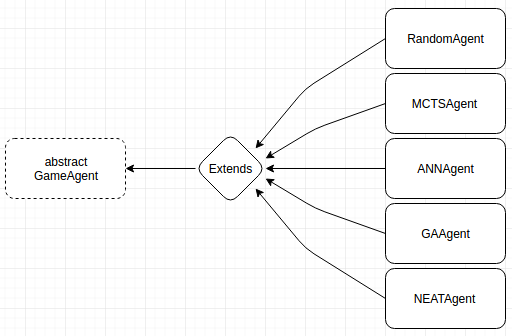
\includegraphics[scale=0.5]{images/gameagent.png}
\caption{Hierarchy of agent implementation}
\label{fig:agentdiag}
\end{figure}

The four non-trivial agents utilize MCTS as the base of their decision-making algorithm, and each have a different Tree policy or Default policy from one another.  Each of the four non-trivial agents follow the four steps of MCTS as outlined in Chapter 1, but each agent may have a slight alteration or addition to the algorithm.  In this section, we describe the way in which we implemented the base MCTS algorithm and \texttt{MCTSAgent}, and then we will look at how each agent modifies this algorithm.  Note that in this next subsection, we will refer solely to the implementation of the \texttt{MCTSAgent} --- however, everything stated directly applies to the other three non-trivial agents as well unless directly stated otherwise when discussing the modified agent.

\subsection{Implementing Monte-Carlo Tree Search}
The main function of MCTS involves incrementally building a tree of possible moves within the game.  For this, we created a \texttt{Node.java} class which behaves slightly differently from how one may expect a generic tree-node to, since it must seperate the children which have been visited in MCTS from those which have not.  Each \texttt{Node} object has the following instance variables:
\begin{itemize}
\item \texttt{double score}\\
Tracks the number of random playouts from this node resulting in a win
\item \texttt{double games}\\
Tracks total number of random playouts performed from this node
\item \texttt{ArrayList$<$Node$>$ unvisitedChildren}\\
Contains all children which have not been visited by MCTS
\item \texttt{ArrayList$<$Node$>$ children}\\
Contains all children which have been visited by MCTS
\item \texttt{ArrayList$<$Node$>$ prunedChildren}\\
Contains nodes pruned (only applicable for ANNAgent)
\item \texttt{Node parent}\\
Points to node's parent
\item \texttt{Board b}\\
The \texttt{Board} associated with the node
\item \texttt{boolean firstPlayer}\\
Tracks who's turn it is on the \texttt{Board} represented by the node
\end{itemize}

\texttt{Node.java} has two constructors, one for the root node of the tree (which is only called on the first iteration of MCTS each turn), and one to create all other nodes.  The root constructor takes a \texttt{Board b} and \texttt{boolean firstPlayer} as arguments and sets the respective instance variables to these values; \texttt{score} is set to 0.0, \texttt{games} is set to 1.0, the children ArrayList is initialized, and its parent is set to \texttt{null}.  The other constructor takes a \texttt{Board b} and \texttt{Node parent} as arguments, and sets the respective instance variables to these.  The only other difference from the root constructor is \texttt{firstPlayer} is set to the opposite of its parent's value.  Each \texttt{Node} has instance methods to find and set its unvisited children, recursively backpropogate scores from random playouts up the tree to the root node, find the UCT value of a node (given an exploration bias parameter as described in Equation \ref{eq:UCT}), and prune nodes from the tree (i.e. remove them from children and/or unvisitedChildren).

Utilizing the \texttt{Node} object, the \texttt{MCTSAgent} is able to build a game tree using MCTS as described in Chapter 1.  In addition to all the instance variables defined in \texttt{GameAgent}, the \texttt{MCTSAgent} also has a \texttt{double explorationConstant} for use in the MCTS algorithm --- for our experiments, this constant was set to $\sqrt{2}$ which provides a rather equal balance between exploration and exploitation \cite{browne2012survey}.  Its \texttt{makeMove} method takes a \texttt{Board b}, \texttt{int timeAllowed}, and  \texttt{int moveNumber} as arguments, which are the current Board, amount of time it is allowed to take to decide on a move, and how many moves have been made in the current game (which is used for random playouts), respectively.

Within the \texttt{makeMove} method is a while-loop which repeatedly calls the agent's \texttt{select} method over its given time allowance.  This method runs through a single iteration of MCTS using various other helper methods --- it selects the node in the tree with the highest UCT value, visits a random one of the node's unvisited children, finds the score of a random playout, and backpropogates it the score up the tree.  Note that with our chosen scoring scheme for Go, the scores of the random playouts can theoretically fall anywhere in the interval $[-s, s]$ where $s$ is the number of cells on the board (e.g. a 9x9 board can have scores anywhere from -81 to 81); however, UCT requires estimated node scores to be in the interval $[0,1]$ \cite{browne2012survey}.  Furthermore, for player two, lower scores are better.  Thus after finding the score of a random playout from a node, we must alter the score before backpropogating it up the tree.

This was a simple process.  First, if the player performing the random playout was the second player, we multiplied the estimated score of the playout by -1.  Then the score was normalized using Equation \ref{eq:norm}, where $s$ is the score of the game on a $b\times b$ Go board.  $s'$ is then the score which is backpropogated up the tree.

\begin{equation}\label{eq:norm}
s' = \frac{s + b^2}{2b^2}
\end{equation}

After the agent spent its alotted amount of time searching the tree, it makes its final move selection.  For final move selection, the agent simply chooses the child of the root with the highest average playout score (i.e. the child with the highest score divided by total games).

\subsection{ANNAgent}
The \texttt{ANNAgent} behaves exactly the same as the \texttt{MCTSAgent} with one caveat: prior to building the game tree with MCTS, it prunes a number of the root's immediate children from the tree.  This is done by training a simple feed-forward network to rank a node's children in order of how likely they are to be repeatedly visited by MCTS --- those with the lowest scores are not included in the search process.  An exponentially decaying pruning scheme is used as outlined in \cite{annpruning}, meaning the number of nodes pruned from the tree exponentially decays as the game progresses.  Using equation \ref{eq:prune} to determine the number of nodes to prune, the agent removes 50 percent of children at move 0, 10 percent of children by move 70, 4 percent by move 125, etc.

\begin{equation}\label{eq:prune}
(\textrm{\% pruned}) = 50 - 48.6*(1 - e^{(-0.0244*x)})
\end{equation}

Seperate neural networks were created and trained for each boardsize of both Go and Hex prior to any experimentation.  In total, 8 neural networks were made (9x9, 11x11, and 14x14 Hex; 5x5, 7x7, 9x9, 11x11, and 13x13 Go).  For this, the Encog machine learning library was used \cite{encog}.  The neural networks were designed as follows for each game on each $n\times n$ board:
\begin{itemize}
\item Input layer consisting of $n\times n$ neurons --- each neuron corresponds to exactly one spot on a board;
\item A single hidden layer consisting of the number of neurons in the input layer divided by 3;
\item Output layer consisting of a single neuron, representing the estimated value of the input board.
\end{itemize}

Only sigmoid activation functions were used in the neural networks, as this was found to provide the best performance for evaluating Go boards by Burger \etal \cite{annpruning}.  We chose a single hidden layer as Heaton, the creator of Encog, suggests that more than a single layer is completely unnecessary for training simple feed-forward networks \cite{encog}.  Finally, we settled on the size of the hidden layer empirically, by briefly testing several hidden layer sizes between that of the input size and output size.

After designing the networks, each network was trained on a seperate set of 2500 randomly generated boards of the network's respective game type and board size.  Each set contained an equal number of boards representing random games after 5 moves, 10 moves, 15 moves, etc. up to 105 moves.  In order to estimate the value of each of these boards, an \texttt{MCTSAgent} performed 10,000 iterations of MCTS for each board; the UCT value of each board after 10,000 iterations was used as the ideal output value for the input board.  

We chose to train each network on this dataset until the network's error was below 0.0001 --- this seems like an incredibly low amount of error, but such a low error was actually necessary to guarantee any level of accuracy from our networks.  Because of our randomly generated inputs for each dataset and the large number of MCTS iterations, most of the ideal values were found to be between 0.45 and 0.55.  Such a small range in most of the training data meant that a calculated level of error would in actuality be magnitudes higher.  For example, if the network were to classify every single input as having a value of 0.5, the error would likely only read to be around 0.05 since most of the ideal values are between 0.45 and 0.55 --- such a network is clearly far from being accurate, despite having a seemingly low error over the training set.

After being trained, the networks were each serialized using Java's serialization library.  The \texttt{ANNAgent} has a \texttt{BasicNetwork} instance variable (imported from the Encog library) which is initialized upon creation of the agent.  Before gameplay, the agent chooses the appropriate network to deserialize based on the gametype and size of the game board.  On each turn, the agent then uses this network to evaluate moves and remove a percentage of them from the game tree, as described earlier.

The process of evaluating each child of the current board, sorting them by estimated ranking, and removing a set number of them from the tree obviously takes some of the agent's alotted time that could be spent performing more iterations of MCTS.  So, what is expected to be gained by this process?  Essentially, the idea behind the \texttt{ANNAgent} is that, while it performs a lower number of iterations of MCTS, more of the iterations it does perform will be done exploring high quality moves.  If we can identify which children will not be explored heavily before even starting MCTS, the number of iterations lost from time spent evaluating children may be overcome by the fact that any iterations of MCTS that would have been wasted exploring those moves can now be spent on deciding between fewer, better options.


\subsection{GAAgent}
The \texttt{GAAgent} utilizes a genetic algorithm to bias both its tree policy and its final move selection.  The agent's genetic algorithm consists of a population of \texttt{GAWeight} objects, which each hold a weight vector of five doubles $(x_1 \cdots x_5)$ between zero and one to represent the weight given to a hueristic property of the game board.  Tables \ref{table:go} and \ref{table:hex} give the names and descriptions of each of the games' heuristic properties which are used.  Each \texttt{GAWeight} also contains methods to evaluate each heuristic property of a given board.

\begin{table}[h]
\centering
\begin{tabular}{|c|l|}
\hline
\textbf{Property name} & \textbf{Definition}\\
\hline
\hline
netStones & Score of resulting board\\\hline
goodLibs & Number of own liberties on board\\\hline
badLibs & Number of opponent's liberties on board\\\hline
goodAtari & Number of own stones in atari\\\hline
badAtari & Number of opponent's stones in atari \\\hline
\end{tabular}
\caption{Properties used for Go genetic algorithm}
\label{table:go}
\end{table}

\begin{table}[h]
\centering
\begin{tabular}{|c|l|}
\hline
\textbf{Property name} & \textbf{Definition}\\
\hline
\hline
netBridges & Net number of bridges on board\\\hline
goodConnected & Size of largest connected region of own stones\\\hline
badConnected & Size of largest connected region of opponent's stones\\\hline
goodDeepest & The smallest number of agent's moves needed to win\\\hline
badDeepest & The smallest number of opponent's moves needed to win\\\hline
\end{tabular}
\caption{Properties used for Hex genetic algorithm}
\label{table:hex}
\end{table}

For example, consider Figures \ref{fig:goheur} and \ref{fig:hexheur}.  These are representations of small boards from Go and Hex, after several moves have been made --- the boards were generated using GoGui \cite{fuego} and HexGui \cite{benzene}, respectively.  On the Go board, the blue dots represent white stones' liberties while the red dots represent black stones' liberties; stones marked with green dots represent stones in atari.  Meanwhile on the Hex board, the blue shaded region represents the largest region of black stones, the red shaded region represents the largest region of white stones, green lines represent any bridges, and the empty spaces marked with `X' represent the spaces where either player would need to play to end the game.

\begin{figure}[h]
\centering
\begin{minipage}{.5\textwidth}
  \centering
  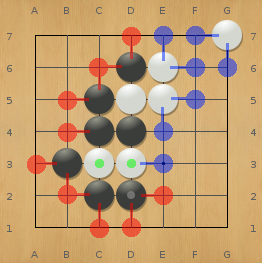
\includegraphics[scale=0.65]{images/goheuredited.png}
  \captionof{figure}{Go heuristic properties}
  \label{fig:goheur}
\end{minipage}%
\begin{minipage}{.5\textwidth}
  \centering
  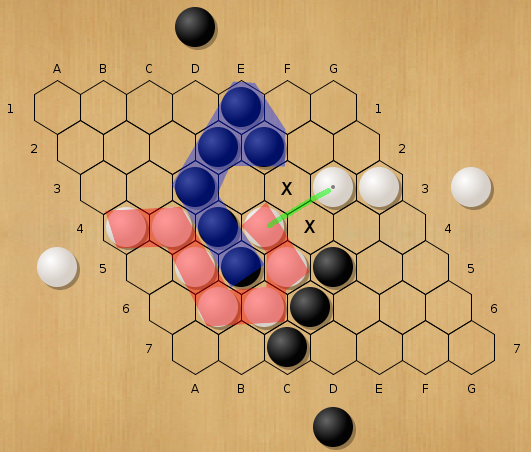
\includegraphics[scale=0.375]{images/hexheuredited.png}
  \captionof{figure}{Hex heuristic properties}
  \label{fig:hexheur}
\end{minipage}
\end{figure}

So, suppose a \texttt{GAAgent} is playing as black in both of these games and one of its \texttt{GAWeights} is evaluating the boards.  For Go, the \texttt{GAWeight} would find a netStones value of -1 (6 white stones and 7 black stones), a goodLibs value of 9, a badLibs value of 7, a goodAtari value of 0, and a badAtari value of 2.  If $(x_1, \cdots, x_5)$ are the respective weights for each property, the \texttt{GAWeight} would find the overall value $v_1$ of the Go board to be 
\[v_1 = -1x_1 + 9x_2 + 7x_3 + 0x_4 + 2x_5.\]
For the Hex board, the \texttt{GAWeight} would find a netBridges value of 1 (1 white bridge and 0 black bridges), a goodConnected value of 6, a badConnected value of 7, a goodDeepest value of 2 (both spots marked x needed to win for black), and a badDeepest value of 1 (only one spot marked x needed to win for white).  So, the \texttt{GAWeight} would find the overall value $v_2$ of the Hex board to be
\[v_2 = 1x_1 + 6x_2 + 7x_3 + 2x_4 + 1x_5.\]

When a \texttt{GAAgent} is created before the start of a game, it is given a small population of 10 \texttt{GAWeights} with randomized weight vectors $(x_1 \cdots x_5)$.  While, traditionally, a genetic algorithm requires each member to fully complete its task (e.g. play a full game of Go) in order to evaluate a member's fitness, the nature of MCTS allows us to to evolve the weight vectors many times during a single game \cite{lucas2014fast} --- rather than use a full, real playout of a game the fitness of a \texttt{GAWeight}, we can use the simulated playouts of a game during each iteration of MCTS.

We evaluate, select, crossover, and mutate the population of \texttt{GAWeights} after every 100 iterations of MCTS; each of the ten \texttt{GAWeights} is used ten times to bias the \texttt{GAAgent} before evaluation.  So, when the \texttt{GAAgent} is asked to make a move, it selects a node of the tree to expand taking into account both the UCT scores and estimated board values of each node.  A random playout is performed from the chosen node as usual, and, for the purpose of fitness evaluation, the score of the playout is stored in whichever \texttt{GAWeight} was used.  After every 100 iterations of MCTS, each \texttt{GAWeight} will have been used 10 times and we can perform the evolutionary algorithm on the population.

Evaluating the fitness of the population is simple; we look at the saved playout scores of each \texttt{GAWeight}, and a higher average score equates to a higher fitness.  The two \texttt{GAweights} with the lowest fitness are removed from the population and are replaced by two children of the highest performing \texttt{GAWeights}.  These children are made by simply averaging the weight vectors of the parents --- prior to mutation, the two children are exactly the same.  Mutation of each child is done independently on each of its weights --- if a weight is chosen to be mutated, it is averaged with a random double between 0 and 1.

For the first child, each weight has a 20\% chance of being mutated, while each weight of the second child has a 60\% chance of being mutated.  So, on average, one of the first child's weights will be mutated while three of the second child's weights will be mutated.  We chose these high mutation rates because of the small population size and the small number of random playouts performed relative to the branching factor of each game.  A high mutation rate keeps the population diverse and allows the agent to more easily discover heuristic strategies far different from those in the starting population.

After the \texttt{GAAgent}'s alotted time to decide on a move is up, it biases its final move selection as well.  The agent assigns a score to each possible move in the same way as the \texttt{MCTSAgent}, biases each move with the highest performing \texttt{GAWeight} in its population, and selects the move with the highest final score.  During both the selction phase of MCTS and final move selection, the \texttt{GAAgent} essentially introduces a small amount of heuristic analysis into its decision making in order to differentiate between nodes in the tree with similar UCT scores.  We observed that during MCTS, there are oftentimes several clusters of nodes which have similar UCT scores.  Hypothetically, the \texttt{GAAgent} should be able to choose between similarly scoring moves more accurately; this could be particularly helpful when the agent is only able to run through a small number of iterations of MCTS (e.g. early in a game of Go on one of the larger boards).

\subsection{NEATAgent}
Rather than alter the MCTS tree policy or final move selection like the previous agents, the \texttt{NEATAgent} uses an evoloved neural network to alter the default policy of MCTS as proposed by Gauci and Stanley in \cite{hyperneatgo}.  The logic behind this agent is that, when playing against a non-trivial player, a random playout will likely not result in a very accurate representation of a game playout.  Thus, a default policy which chooses moves more intelligently will allow the MCTS algorithm to better estimate the scores of playouts during the simulation phase.

Gauci and Stanley proposed using NEAT to create a network which acts as an action selector --- given a board, the network provides each empty space with a score based on how valuable placing a piece at that spot would be.  The Encog framework \cite{encog} provides NEAT functionality and was used to implement this system.  Similar to the ANNs created for \cite{ANNAgent}, a different network was created for each boardsize of each game, and each have an input layer size equal to the number of spots on the board (e.g, 81 input neurons for a game on a 9x9 board).  Because these networks are acting as an action selector, the size of the output layer is also equal to the number of spots on the board --- each output neuron represents the value of placing a piece at the spot represented by the input neuron in the same place.  The networks were limited to using only sigmoid activation functions.

To train the networks, we again randomly generated 2500 boards of the appropriate game and board size for each.  For each board, an \texttt{MCTSAgent} performed 5000 iterations of MCTS using the board as the root of the tree.  This allowed us to estimate the value of each legal move by looking at the score of each of the board's children.  The ideal value for the output of the board was set to the corresponding move's score; any output neurons which represented spaces which were not valid moves had the ideal value set to 0.  

After the training dataset was created, each network was trained until its error was below 0.1.  The networks were then serialized using Java's serialization library, and the \texttt{NEATAgent} contains a \texttt{NEATNetwork} instance variable, similar to the \texttt{ANNAgent}.  Upon creation, the \texttt{NEATAgent} can pick the appropriate network to use, and assign the network to this instance variable.  During MCTS, the \texttt{NEATAgent} has a standard selection and expansion phase.  For the simulation phase, though, the agent uses a built-in playout method called \texttt{biasedPlayout} rather than the random playout functionality provided in the games classes.

The \texttt{biasedPlayout} method takes a \texttt{Node} as input (the node which is expanded to during MCTS), and returns a score of a playout from this \texttt{Node}.  During each move of the simulated playout, the agent evaluates the current board with its network and places a piece at the spot corresponding to the output neuron with the highest value.  The agent's MCTS process is otherwise the same as the standard \texttt{MCTSAgent}, calculating the score at the end of the playout and backpropogating it up the tree.  The agent's final move selection is also the same, selecting the move with the highest ratio of average-playout-score to total-games-simulated.

\section{Games Framework}
\texttt{GameController.java} is the ``runner'' class of our framework and orchestrates the actual playing of games --- it is used to create game and agent objects, run the games, and record data.  In order to run this program, note that you must include the \texttt{encog-core-3.3.0} and \texttt{jcommander-1.48} JARs included in the \texttt{/lib} directory of the project.  The class contains a \texttt{Game} object, a \texttt{Board} object which acts as the master game board, two \texttt{GameAgent} objects, and several \texttt{FileWriters} to record data.  We parse command-line inputs using the JCommander library \cite{jcommander} to determine gametype, board size, which agents are playing, etc. (Table \ref{table:jco}).  Our framework also supports human play by printing the game board to the terminal between moves, and allowing human players to make moves by typing the row and column of the space on which they wish to place their piece.

\begin{table}[h]
\centering
\begin{tabular}{|l|c|l|}
\hline
\textbf{Parameter} & \textbf{Default} & \textbf{Description}\\
\hline
\hline
String --agent1 & ``human" & Player one's agent type \\\hline
String --agent2 & ``human" & Player two's agent type \\\hline
int --size & 9 &  Size of the game board\\\hline
String --game & ``go" & The game being played \\\hline
int --time & 3000 & How many milliseconds can be spent making a move \\\hline
boolean --record & false & Record game data \\\hline
boolean --help & false & Display JCommander usage \\\hline 
\end{tabular}
\caption{JCommander parameters for \texttt{GameController.java}}
\label{table:jco}
\end{table}

Following the creation of all of the necessary objects, \texttt{GameController} simply enters a \texttt{while-loop} which executes until the game is complete; the game over condition for whichever game is being played is checked following every move.  While the game over condition is not met, each of the two players are simply asked to make a move.  If the player is human, the game halts until a valid move is typed into the terminal; otherwise, the agent's \texttt{makeMove} method is called for the current \texttt{Board}, movenumber, and time allowance.  After each move, if \texttt{--record} has been set to true, the current game score and number of iterations of MCTS the agent was able to complete (if applicable) is written to a .csv file.  Figure \ref{fig:finalframework} illustrates the entire structure of the framework during gameplay between two agents.

\begin{figure}[h]
\centering
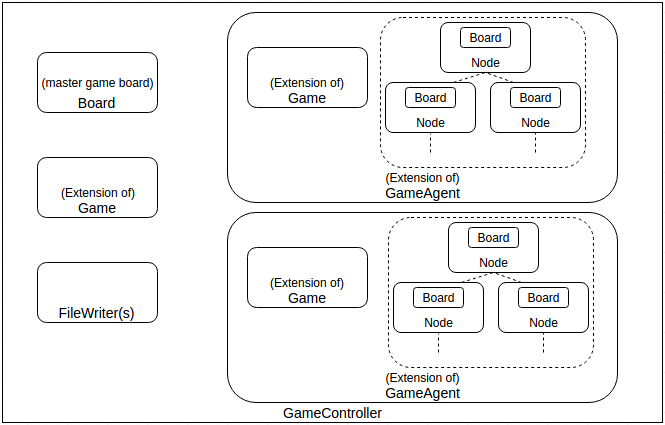
\includegraphics[scale=0.58]{images/finalframework.png}
\caption{Structure of the game-playing framework}
\label{fig:finalframework}
\end{figure}

The entire framework was written with expandability in mind.  The extensive use of object-oriented programming paradigms allows for new games and agents to be integrated into the framework with ease.  Adding support for a new game or agent would require no changes to the existing Java classes, other than adding a few lines to instantiate the new object in \texttt{GameController.java}.

\section{Experiments}
Our experiments consisted of having every agent play one another multiple times on different sized boards of each game under different time allowances.  Each pair of agents played games on 5x5, 7x7, 9x9, 11x11, and 13x13 Go as well as 9x9, 11x11, and 14x14 Hex.  For each of these gametypes, 20 games were played with time allowances of 500ms, 1000ms, 2000ms, 4000ms, and 8000ms.  The goal of running so many variations of the games is to uncover performance trends of each agent relative to one another as the board size and time allowance changes.  The different board sizes provide different branching factors (e.g. 13x13 Go has a much higher branching factor than 7x7 Go), while the different time allowances allow for each agent to run through more iterations of MCTS on each turn.

Because of the large number of experiments, we chose to distribute them over multiple machines in Alden Hall and run them concurrently.  We achieved this by manually \texttt{ssh}ing into a different machine for each pair of agents, and running a simple \texttt{bash} script on each to run 20 games between the two agents for each variation in board size and time allowance.  Each \texttt{bash} script simply sets the classpath to include the necessary JARs, and loops through playing the different games with the \texttt{--record} option set to true.

\section{Threats to Validity}
I think I will have a section on issues with / potential improvements to the project in the final chapter, after the results have been discussed.  That organization makes more sense to me (explain implementation/experiments -$>$ analyze results -$>$ discuss validity of results/improvements to the experiments).  Leaving this here for now so I don't forget about this later if I change my mind. % Chapter organization is topic-dependent

%ch:implem
%
% $Id: ch04_implementation.tex
%
%   *******************************************************************
%   * SEE THE MAIN FILE "AllegThesis.tex" FOR MORE INFORMATION.       *
%   *******************************************************************
%
\chapter{Experimental Results}\label{ch:implem}
Our experiments consisted of having every agent play one another multiple times on different sized boards of each game under different time allowances.  Each pair of agents played games on 5x5, 7x7, 9x9, 11x11, and 13x13 Go as well as 9x9, 11x11, and 14x14 Hex.  For each of these gametypes, 20 games were played with time allowances of 500ms, 1000ms, 2000ms, 4000ms, and 8000ms.  The different board sizes provide different branching factors (e.g. 13x13 Go has a much higher branching factor than 7x7 Go), while the different time allowances allow for each agent to run through more iterations of MCTS on each turn.  In the course of our experiments, we were able to uncover several interesting performance trends.

This chapter is organized by game; there is one section covering the reseults from the Go gameplay, and another on the results from the Hex gameplay.  In each section, we first note the agents' performances against the trivial \texttt{RandomAgent}, then overview the results from each experimental agent's games against \texttt{MCTSAgent}, and then finally look at the head-to-head games between the experimental agents.  Note that due to the size and number of our data visualizations, we will often cite Appendix \ref{appa:data}, which houses all of our data visualizations in full, when referencing data.  While most of the full visualizations will not be in this chapter, some small snippets will be included.  

For some context on the Go score visualizations, consider Figure \ref{fig:ex} as an example.  Each colored line represents the score of a different game of Go, whose size and time allowance is specified at the top of the Figure.  Each line plots the score of a single playout over the course of a 250 move game.  A positive score is a good score for the first player, while a negative score is a good score for the second player --- so here, a positive score is good for \texttt{ANNAgent}, while a negative score is good for \texttt{MCTSAgent}.  The smooth, gray curve shows the overall score across all plays of the game at each move for the given configuration.

\begin{figure}[h]
  \centering
  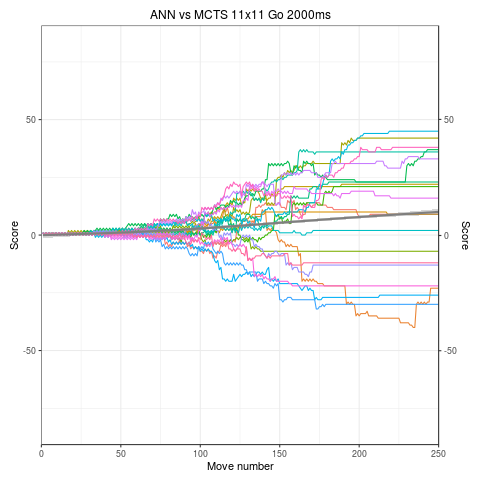
\includegraphics[scale=0.6]{images/Visualizations/ANNvsMCTS/2000ms11x11.png}
  \caption{Example Visualization}
  \label{fig:ex}
\end{figure}
  

\section{Go}
The results of the games between each intelligent agent and the \texttt{RandomAgent} are surprisingly significant.  We assumed each of the intelligent agents would vastly outperform the \texttt{RandomAgent}, and the raw win/loss numbers for these games (Table \ref{tab:ranloss}) seem to indicate exactly this --- each agent won between 98\% and 99\% of their games against the \texttt{RandomAgent}.  However, the plots tracking the game scores over the course of the games tell a different story.  The \texttt{MCTSAgent} and \texttt{ANNAgent} appear to have a normal performance --- they usually take a quick lead and rarely give up points, regardless of board size or time allowance.  This, however, was not the case for the \texttt{GAAgent}.

\begin{table}
\centering
\begin{tabular}{|c|c|c|}
\hline
\textbf{Agent Type} & \textbf{Losses to RandomAgent} & \textbf{Total Games}\\ \hline\hline
\texttt{MCTSAgent} & 5 & 400\\ \hline
\texttt{ANNAgent} & 6 & 400\\ \hline
\texttt{GAAgent} & 7 & 400\\ \hline
\end{tabular}
\caption{Intelligent Agent Losses to \texttt{RandomAgent}}
\label{tab:ranloss}
\end{table}

\begin{figure}[h]
\centering
\begin{minipage}{.45\textwidth}
  \centering
  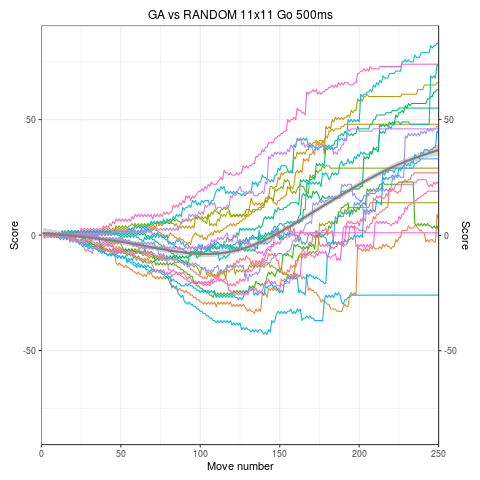
\includegraphics[scale=0.4]{images/Visualizations/GAvsRANDOM/500ms11x11.png}
\end{minipage}%
\begin{minipage}{.45\textwidth}
  \centering
  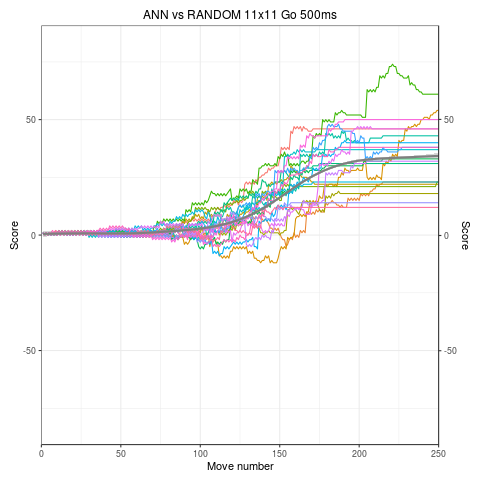
\includegraphics[scale=0.4]{images/Visualizations/ANNvsRANDOM/500ms11x11.png}
\end{minipage}
\caption{\texttt{GAAgent}'s and \texttt{ANNAgent}'s performance against \texttt{RandomAgent}}
\label{fig:rand}
\end{figure}

For large boards and/or a small time allowance, the \texttt{GAAgent} has a tendency to actually fall behind the \texttt{RandomAgent} for a significant portion of the game.  The larger the board and smaller the time allowance, the longer the agent performs poorly; the agent's performance always seems to vastly improve later in the game, though, leading to a seemingly higher performance.  Note the shape of the two graphs in Figure \ref{fig:rand}, which compares the performance of the \texttt{GAAgent} and \texttt{ANNAgent} against the \texttt{RandomAgent}.

The \texttt{GAAgent} only loses a single game of this configuration, even ending with a higher average score than the \texttt{ANNAgent}.  However at turn 150 out of 250, on average the \texttt{GAAgent} is actually losing by a significant amount against the \texttt{RandomAgent}.  Meanwhile the \texttt{ANNAgent} is consistently winning almost all of its games at move 150.  This can be observed happening between other game configurations in Figure \ref{app:garandscore} of Appendix \ref{appa:data}.  This type of performance ended up being a trend for the \texttt{GAAgent}.

\begin{figure}[h]
\centering
\begin{minipage}{.45\textwidth}
  \centering
  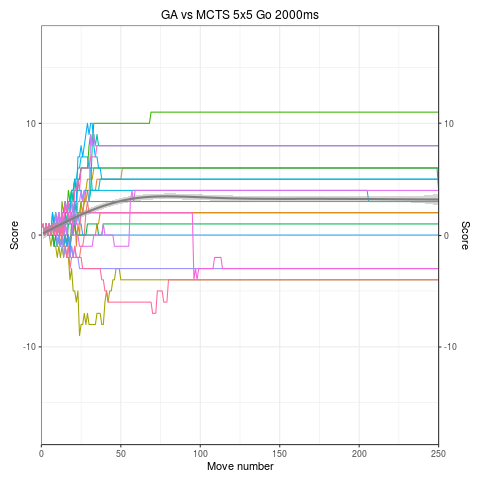
\includegraphics[scale=0.4]{images/Visualizations/GAvsMCTS/2000ms5x5.png}
\end{minipage}%
\begin{minipage}{.45\textwidth}
  \centering
  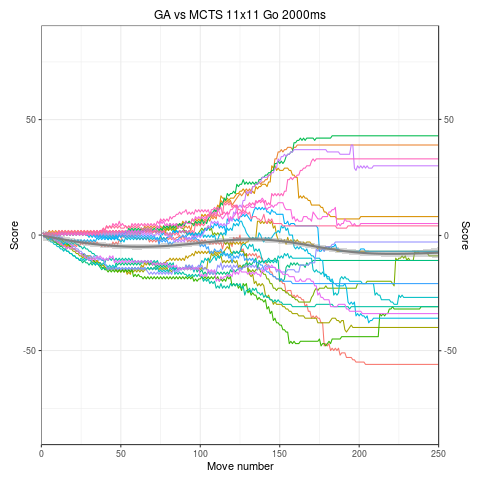
\includegraphics[scale=0.4]{images/Visualizations/GAvsMCTS/2000ms11x11.png}
\end{minipage}
\caption{\texttt{GAAgent} vs \texttt{MCTSAgent} performance on different board sizes}
\label{fig:gamcts}
\end{figure}

The results of the games between \texttt{ANNAgent} and \texttt{MCTSAgent} (Appendix \ref{appa:data} Figure \ref{app:annmctsscore}) are quite conclusive.  The \texttt{ANNAgent} consistently slightly outperforms the \texttt{MCTSAgent} regardless of board size and time allowance.  While the \texttt{MCTSAgent} did manage to win a number of games in each board configuration, we can see that the average score favors the \texttt{ANNAgent} in 18 out of 20 board configurations.  On the two configurations for which the \texttt{ANNAgent} did not outperform the \texttt{MCTSAgent}, the average score was 0, favoring neither agent.

\begin{figure}[h]
\centering
\begin{minipage}{.45\textwidth}
  \centering
  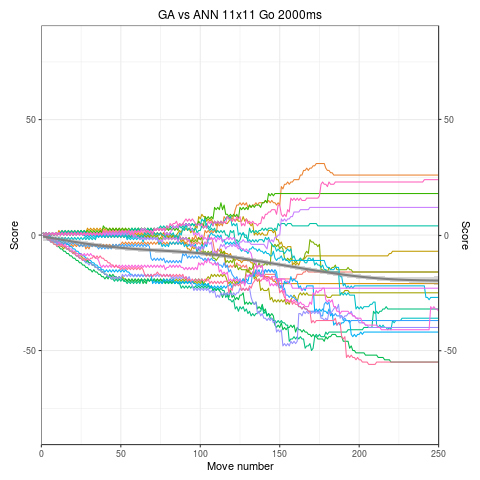
\includegraphics[scale=0.4]{images/Visualizations/GAvsANN/2000ms11x11.png}
\end{minipage}%
\begin{minipage}{.45\textwidth}
  \centering
  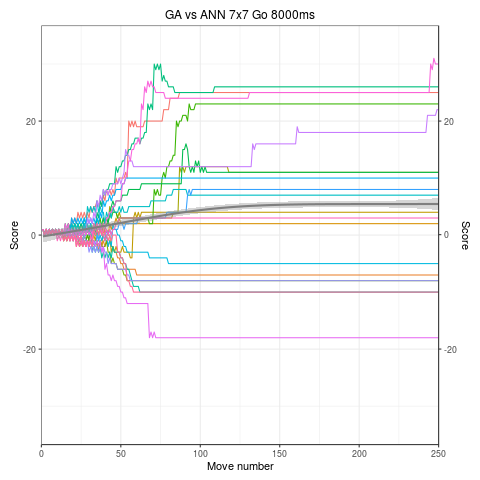
\includegraphics[scale=0.4]{images/Visualizations/GAvsANN/8000ms7x7.png}
\end{minipage}
\caption{\texttt{ANNAgent} and \texttt{GAAgent} on their more dominant board configurations}
\label{fig:gamcts}
\end{figure}

The \texttt{GAAgent}'s results against the \texttt{MCTSAgent} are rather consistent with what was observed against the \texttt{RandomAgent} --- essentially, performance trends upwards as the time allowance increases, and performance trends downwards as board size increases.  An example of this can be seen in Figure \ref{fig:gamcts}, which shows the scores for two board sizes at the same time allowance.  Each row of graphs in Appendix A Figure \ref{appa:gamctsscore} clearly shows this trend --- scores favor \texttt{MCTSAgent} more and more as board size increases.  The \texttt{GAAgent}, though, does tend to outperform the \texttt{MCTSAgent}.  While not as dominant as the \texttt{ANNAgent}, it was able to achieve a higher average score for the majority of board configurations, especially those with smaller boards or higher time allowances.

The head-to-head matchups between \texttt{GAAgent} and \texttt{ANNAgent} provide the most obvious patterns in our data, and further confirms our suspicions about the \texttt{GAAgent}'s performance trend.  The \texttt{GAAgent} was able to achieve a higher average score on every set of games which had either a 5x5 game board (the smallest size used), or a time allowance of 8000ms (the highest time allowance used).  Meanwhile the \texttt{ANNAgent} tended to have a much better performance on boards with a lower time allowance and larger board size, most notably on the 11x11 and 9x9 boards (excluding those with an 8000ms time allowance).

The configurations which had both a moderate board size and moderate time allowance led to the games being somewhat of a tossup between the two agents.  Some configurations saw the \texttt{GAAgent} with the higher average score, while others gave it to the \texttt{ANNAgent}.  In general, the more moderate the board size and time allowance, the closer the average game score tended to 0.

\section{Final Analysis}
The results of the experiments painted a shockingly clear picture.  We found that the \texttt{ANNAgent}'s performance was rather consistent regardless of board size or time allowance. It's tree pruning technique provides a moderate boost in performance over a standard Monte-Carlo Tree Search, and does not noticably change with such changes in board configuration.  This demonstrates the value of having certain nodes in the game tree be visited a higher number of times, even at the expense of a smaller number of overall MCTS iterations.  Because of this, it can be used to reliably improve on MCTS without a need to worry about the structure of the game.

The \texttt{GAAgent} can also provide a demonstrable boost in performance over standard MCTS, but its algorithm's performance is much more dependant on the board size and time allowance it is given.  Its performance has a strong positive correlation with time allowance, and a strong negative correlation with board size.  Overall, this leads its performance to be much more variable.  It can outperform the \texttt{ANNAgent} in some configurations, but in others it can struggle against even the trivial \texttt{RandomAgent}.

We can explain the \texttt{GAAgent}'s performance trend rather easily.  Because of the random starting point of its population of heuristic weights, it requires a large number of iterations through MCTS before its population can find a decent hueristic function.  With a low time allowance or a large board size, it simply cannot find an appropriate heuristic function until rather late in the game.  This does, however, speak to the potential power of this type of agent.  Despite its notably bad performance early on in many games, it was often able to outperform its opponent and win by the end of the game.

The agent, though, is likely very dependant on starting with an appropriate hueristic.  If the things the agent is measuring on the board as its hueristic do not represent a realistic strategy, it is very likely the agent would perform poorly --- its performance may even be lower than a standard MCTS. % Chapter organization is topic-dependent

% YOU MAY HAVE SEVERAL MORE CHAPTERS, DEPENDING ON TOPIC AND ORGANIZATION

%ch:conclusion
%
% $Id: conclusion.tex
%
%   *******************************************************************
%   * SEE THE MAIN FILE "AllegThesis.tex" FOR MORE INFORMATION.       *
%   *******************************************************************
%

\chapter{Summary}\label{ch:conclusion}
\section{Future Work}
Most improvements to our work are needed in the games classes.  Since each agent utilizes methods in the game classes for the MCTS process, any improvements to the algorithms within the games classes will immediately lead to a performance boost in each agent.  The most needed improvement is on the \texttt{boardResolution} method of the Go class.  The algorithm has a very high time-complexity, and is called in every iteration of MCTS; this combination leads to an agent's performance becoming exponentially worse as board size increases.

Beyond this, we would like to test agents with better trained neural networks.  To train each neural network, we used only 2500 pieces of data; this is an admittedly small training set.  These networks were able to provide the agent with a noticeable performance boost, but it would be interesting to see how much better performance would be with a more reliable network.

\section{Conclusion}
We have implemented a new general-purpose game playing framework for two-player turn-based board games.  The framework supports both human and computer players, and is completely uncoupled from any game-specific functionality; new games can be designed and played on the framework with almost no change to the existing codebase.  We also implemented the games Go and Hex for the framework.  We then created one trivial and four intelligent general-purpose game playing agents.  Similar to the entire framework, the agents contain no game-specific functionality and could be used with any games that run on our platform.

The trivial agent is called \texttt{RandomAgent}, and simply performs random moves on the board.  The first intelligent agent is called \texttt{MCTSAgent}, and utilizes Monte-Carlo Tree Search as its decision-making algorithm.  After these agents were implemented, we created the following three agents: \texttt{GAAgent}, \texttt{ANNAgent}, and \texttt{NEATAgent}; for this, we heavily employed the Encog machine learning framework.  Each of these agents utilize their respective machine learning technique to alter the standard MCTS algorithm, following the proposals of several different previous researchers.

We used our framework and game implementations to perform novel research on these agents.  While they're respective algorithms have been compared to a standard MCTS algorithm and were found to improve on its performance, these experiments were often done in different environments and under different conditions.  Furthermore, agents utilizing these algorithms had never before been directly compared to one another --- we provide this direct comparison.  We ran a series of experiments between each agent on the games Go and Hex with a variable board size and MCTS time allowance.  These parameters provide different branching factors for the games, and overall MCTS iteration restrictions, respectively.  Varying these parameters provides the most applicable real-world results.

The data from our experiments uncovered some very clear performance trends.  Particularly, the \texttt{ANNAgent} provided a moderate boost in performance that was independent of both board size and time allowance.  This makes it a reliable choice with which to improve MCTS.  The \texttt{GAAgent}'s performance was more variable.  While it had the potential to provide a higher performance boost than the \texttt{ANNAgent} under certain circumstances, its performance was very weak in others.  Specifically, we found that the \texttt{GAAgent}'s performance had a positive correlation with time allowance, and a negative correlation with board size.

Our research provides new data on an algorithm which is currently heavily used in the field of artificial intelligence.  Beyond this, the framework we have implemented has the potential to make similar future research in this area much more straight-forward. % Conclusion/future work

%   ********************************************************************
%   * IF YOU HAVE ANY APPENDICES (FOR INSTANCE, CODE, DATA, GRAPHS,    *
%   * OR ANYTHING ELSE THAT DOESN'T "FIT" AS REGULAR CHAPTER CONTENT), *
%   * INCLUDE THE FOLLOWING LINE, WHICH INSTRUCTS LATEX TO CHANGE FROM *
%   * NUMBERED "CHAPTER" HEADINGS TO LETTERED "APPENDIX" HEADINGS.     *
%   *                                                                  *
%   * APPENDICES HAVE THE SAME FORMATTING COMMANDS AS CHAPTERS (E.G.,  *
%   * "\chapter{...}", "\section{...}", ETC.)                          *
%   ********************************************************************

\appendix

%
% $Id: appa--code
%
%   *******************************************************************
%   * SEE THE MAIN FILE "AllegThesis.tex" FOR MORE INFORMATION.       *
%   *******************************************************************

\chapter{Java Code}\label{appa:code}
All program code should be fully commented. Authorship
of all parts of the code should be clearly specified. 

%   *******************************************************************
%   * SEE THE MAIN FILE "AllegThesis.tex" FOR THE "\lstset" COMMAND   *
%   * THAT DEFINES HOW PROGRAM LISTINGS WILL LOOK.                    *
%   *******************************************************************


\lstinputlisting[caption=ANNAgent.java]{../src/ANNAgent.java}

\lstinputlisting[caption=Board.java]{../src/Board.java}

\lstinputlisting[caption=GAAgent.java]{../src/GAAgent.java}

\lstinputlisting[caption=GAWeight.java]{../src/GAWeight.java}

\lstinputlisting[caption=Game.java]{../src/Game.java}

\lstinputlisting[caption=GameAgent.java]{../src/GameAgent.java}

\lstinputlisting[caption=GameController.java]{../src/GameController.java}

\lstinputlisting[caption=GoGame.java]{../src/GoGame.java}

\lstinputlisting[caption=JCommanderInput.java]{../src/JCommanderInput.java}

\lstinputlisting[caption=MCTSAgent.java]{../src/MCTSAgent.java}

\lstinputlisting[caption=NEATAgent.java]{../src/NEATAgent.java}

\lstinputlisting[caption=NEATTrainer.java]{../src/NEATTrainer.java}

\lstinputlisting[caption=NetworkTrainer.java]{../src/NetworkTrainer.java}

\lstinputlisting[caption=NNTest.java]{../src/NNTest.java}

\lstinputlisting[caption=Node.java]{../src/Node.java}

\lstinputlisting[caption=Pair.java]{../src/Pair.java}

\lstinputlisting[caption=Queue.java]{../src/Queue.java}

\lstinputlisting[caption=RandomAgent.java]{../src/RandomAgent.java}

\lstinputlisting[caption=TestNetworks.java]{../src/TestNetworks.java}  % Appendices go here

%   ********************************************************************
%   * THE FINAL COMMANDS DEAL WITH BIBLIOGRAPHY/REFERENCES. IF THERE   *
%   * ARE ANY ITEMS IN YOUR BIBTEX FILE THAT YOU DID NOT REFERENCE IN  *
%   * YOUR PAPER, BUT THAT YOU WISH TO INCLUDE IN THE BIBLIOGRAPHY,    *
%   * YOU MAY SPECIFY "\nocite" COMMANDS TO FORCE THEM TO BE INCLUDED. *
%   *                                                                  *
%   * THE COMMAND "\nocite{*}" FORCES EVERY ITEM IN YOUR BIBTEX FILE.  *
%   ********************************************************************

%\nocite{ckm-acmap-99}   % EXAMPLES OF FORCING THINGS TO BE INCLUDED
%\nocite{Dierckx93}      %   "   "   "
%\nocite{obs-stcav-92}   %   "   "   "
%\nocite{bb4471}         %   "   "   "

\nocite{*} % OR DO THIS TO INCLUDE ALL BIBTEX REFERENCES IN THE BIBLIOGRAPHY

%\bibliographystyle{plain}

%   ********************************************************************
%   * IF YOU HAVE YOUR BIBLIOGRAPHY IN A SEPARATE ".bib" FILE, HERE IS *
%   * WHERE YOU MUST SPECIFY IT. IN THIS EXAMPLE, THE BIBLIOGRAPHY     *
%   * ENTRIES ARE STORED IN A SUBDIRECTORY NAMED "Bibdir" IN A FILE    *
%   * NAMED "myBibtexDB.bib".                                          *
%   ********************************************************************

\bibliographystyle{plain}
%\bibliography{senior_thesis_proposal}
\newpage  
\begin{thebibliography}{99}
\bibitem{imagenet} Krizhevsky, Alex; Sutskever, Ilya; Hinton, Geoffrey E.; \emph{ImageNet Classification with Deep Convolutional Neural Networks}, Advances in neural information processing systems, IEEE, 2012.

\bibitem{HintonDeng} Hinton, Geoffrey; Deng, Li; Yu, Dong; Dahl, George; Mohamed, Abdel-rahman; Jaitly, Navdeep; Senior, Andrew; Vanhoucke, Vincent; Nguyen, Patrick; Sainath, Tara; Kingsbury, Brian; \emph{Deep Neural Networks for Acoustic Modeling in Speech Recognition},  IEEE Signal Processing Magazine, Pearson Education, 2012.

\bibitem{parkhi15} Parkhi, Omkar M.; Vedaldi, Andrea; Zisserman, Andrew; \emph{Deep Face Recognition}, Robotics Research Group, 2015.

\bibitem{wavenet} Van den Oord, Aaron; Dieleman, Sander; Zen, Heiga; Simonyan, Karen; Vinyals, Oriol; Graves, Alex; Kalchbrenner, Nal; Senior, Andrew; Kavukcuoglu, Koray; \emph{WaveNet: A Generative Model for Raw Audio}, Google DeepMind, 2016.

\bibitem{robocup} RoboCup Soccer Tournament, \url{http://www.robocup2016.org/en/}.

\bibitem{Gunderson} Gunderson, Louise F.; Gunderson, James P.; \emph{Robots, Reasoning, and Reification}, Springer, 2008

\bibitem{Bihlmaier} Bihlmaier, Andreas; Worn, Heinz; \emph{Robot Unit Testing}, Proceedings of the 4th International Conference on Simulation, Modeling, and Programming for Autonomous Robots, ACM, 2014

\bibitem{Policonomics} \url{http://www.policonomics.com/perfect-imperfect-information/}, Policonomics, 2012

\bibitem{Gilpin} Gilpin, Andrew; Sandholm, Tuomas; \emph{Lossless abstraction of imperfect information games}, ACM, 2007

\bibitem{minimax} Flying Machine Studios, \emph{An Exhaustive Explanation of Minimax, a Staple AI Algorithm}, \url{http://www.flyingmachinestudios.com/programming/minimax/}, 2012

\bibitem{chaslot2008monte} Chaslot, Guillaume; Bakkes, Sander; Szita, Istvan; Spronck, Pieter; \emph{Monte-Carlo Tree Search: A New Framework for Game AI}, AIIDE, 2008

\bibitem{Trompfinal} Tromp, John; Farenback, Gunnar; \emph{Combinatorics of Go}, Lecture Notes in Computer Science, Vol. 4630, Springer, 2016

\bibitem{alphago} David Silver, Aja Huang, Chris J. Maddison, Arthur Guez, Laurent Sifre, George van den Driessche, Julian Schrittwieser, Ioannis Antonoglou, Veda Panneershelvam, Marc Lanctot, Sander Dieleman, Dominik Grewe, John Nham, Nal Kalchbrenner, Ilya Sutskever, Timothy Lillicrap, Madeleine Leach, Koray Kavukcuoglu, Thore Graepel, Demis Hassabis, \emph{Mastering the Game of Go with Deep Neural Networks and Tree Search}, Nature, 2016

\bibitem{benzene} Henderson, Philip Thomas, \emph{Playing and Solving the Game of Hex}, University of Alberta, 2010

\bibitem{goscore} Hollosi, Arno; Pahle, Morten, \emph{Sensei's Library: Scoring}, \url{http://senseis.xmp.net/?Scoring}, 2017

\bibitem{browne2012survey} Browne, Cameron B;; Powley, Edward; Whitehouse, Daniel; Lucas, Simon M; Cowling, Peter I; Rohlfshagen, Philipp; Tavener, Stephen; Perez, Diego; Samothrakis, Spyridon; Colton, Simon; \emph{A survey of monte carlo tree search methods}, Computational Intelligence and AI in Games, IEEE, 2012

\bibitem{lucas2014fast} Lucas, Simon M; Samothrakis, Spyridon; Perez, Diego; \emph{Fast evolutionary adaptation for monte carlo tree search}, Applications of Evolutionary Computation, Springer, 2014

\bibitem{audibert2009exploration} Audibert, Jean-Yves; Munos, R{\'e}mi; Szepesv{\'a}ri, Csaba; \emph{Exploration--exploitation tradeoff using variance estimates in multi-armed bandits}, Theoretical Computer Science, Elsevier, 2009

\bibitem{nakhost2009monte} Nakhost, Hootan and M{\"u}ller, Martin, \emph{Monte-Carlo Exploration for Deterministic Planning}, IJCAI, 2009

\bibitem{fuego} Enzenberger, Markus; M{\"u}ller, Martin; Arneson, Broderick; Segal, Richard; \emph{Fuego—an open-source framework for board games and Go engine based on Monte Carlo tree search}, Computational Intelligence and AI in Games, IEEE, 2010

\bibitem{fuzzymitchell99} Melanie, Mitchell, \emph{An Introduction to Genetic Algorithms},  MIT Press, 1999

\bibitem{rave} Silver, David, \emph{Monte-Carlo Tree Search and Rapid Action Value
Estimation in Computer Go}, Elsevier, 2011

\bibitem{Cazenave2007} Cazenave, Tristan, \emph{Evolving Monte Carlo tree search algorithms}, L.I.A.S.D., 2007

\bibitem{aimodern} Russell, Stuart and Norvig, Peter \emph{Artificial Intelligence: A Modern Approach}, 3rd ed., Prentice Hall, 2009

\bibitem{pruningsource7} Engelbrecht, A. P., \emph{Computational Intelligence: An Introduction}, 2nd ed., Wiley Publishing, 2007

\bibitem{annpruning} Burger, Clayton; Plessis, Mathys C. du; Cilliers, Charmain B.; \emph{Design and Parametric Considerations for Artificial Neural Network Pruning in UCT Game Playing}, SAICSIT 2013, ACM, 2013

\bibitem{NEAT} Stanley, Kenneth O. and Miikkulainen, Risto, \emph{Evolving Neural Networks through Augmenting Topologies}, Evolutionary Computation, MIT Press, 2002

\bibitem{HyperNEAT} Stanley, Kenneth O.; D;Ambrosio, David; Gauci, Jason; \emph{A Hypercube-Based Indirect Encoding for Evolving Large-Scale Neural Networks}, Artificial Life Journal, MIT Press, 2009

\bibitem{hyperneatgo} Gauci, Jason and Stanley, Kenneth O. \emph{Indirect Encoding of Neural Networks for Scalable Go}, PPSN 2010, MIT Press, 2010

\bibitem{handwriting} Nielsen, Michael A., \emph{Neural Networks and Deep Learning}, Determination Press, 2015

\bibitem{hyperpic} ES-HyperNEAT, \url{http://eplex.cs.ucf.edu/ESHyperNEAT/}, 2012

\bibitem{clarifai} Clarifai visual recognition, \url{https://www.clarifai.com/technology}, 2016

\bibitem{lemoine} Lemoine, Julien and Viennot, Simon, \emph{Computer analysis of Sprouts with nimbers}, Games of No Chance 4, MSRI, 2015

\bibitem{Marcolino} Marcolino, L.S. and Matsubara, H., \emph{Multi-Agent Monte Carlo Go},  Proceedings of the Tenth International Conference on Autonomous Agents and Multiagent Systems, 2011

\bibitem{Takeuchi} S. Takeuchi, T. Kaneko, and K. Yamaguchi, \emph{Evaluation of Monte Carlo Tree Search and the Application to Go}, CIG 08, 2008

\bibitem{computergoevents} Computer Go --- Past Events, \url{http://www.computer-go.info/events/}, 2016

\bibitem{hexwiki} Jean-Luc, W. \emph{Wining situation on a Hex Board}, 2009

\bibitem{sproutstree} Cornell Math Explorer's Club, \url{http://www.math.cornell.edu/mec/2003-2004/graphtheory/sprouts/sproutsgametree.html}, 2003

\bibitem{gostats} \emph{Length of a Go Game}, \url{http://homepages.cwi.nl/~aeb/go/misc/gostat.html}

\bibitem{leemon} Baird, Leemon and Schweitzer, Dino, \emph{Complexity of the Game of Sprouts}, 2010

\bibitem{torbert} Torbert, Shane, \emph{Applied Computer Science}, 2nd Ed., Springer, 2012

\bibitem{encog} Heaton, Jeff, \emph{Encog: library of interchangeable machine learning models for Java and C\#}, Journal of Machine Learning Research, Volume 16, 2015 

\bibitem{jcommander} Beust, Cedric, \emph{Jcommander command line parsing framework}, 2017

\bibitem{encogref1} Menden, Michael P and Iorio, Francesco and Garnett, Mathew and McDermott, Ultan and Benes, Cyril H and Ballester, Pedro J and Saez-Rodriguez, Julio, \emph{Machine learning prediction of cancer cell sensitivity to drugs based on genomic and chemical properties}, PLoS one, 2013

\bibitem{encogref2} Awan, Shahid M and Aslam, Muhammad and Khan, Zubair A and Saeed, Hassan, \emph{An efficient model based on artificial bee colony optimization algorithm with Neural Networks for electric load forecasting}, Neural Computing and Applications, Springer, 2014

\bibitem{encogref3} Ramos-Poll{\'a}n, Ra{\'u}l and Guevara-L{\'o}pez, Miguel {\'A}ngel and Oliveira, Eug{\'e}nio, \emph{A software framework for building biomedical machine learning classifiers through grid computing resources}, Journal of medical systems, Springer, 2012

\end{thebibliography}

%\begin{spacing}{1}
%\bibliographystyle{plain}
%\bibliography{senior_thesis_proposal}
\newpage  
\begin{thebibliography}{99}
\bibitem{imagenet} Krizhevsky, Alex; Sutskever, Ilya; Hinton, Geoffrey E.; \emph{ImageNet Classification with Deep Convolutional Neural Networks}, Advances in neural information processing systems, IEEE, 2012.

\bibitem{HintonDeng} Hinton, Geoffrey; Deng, Li; Yu, Dong; Dahl, George; Mohamed, Abdel-rahman; Jaitly, Navdeep; Senior, Andrew; Vanhoucke, Vincent; Nguyen, Patrick; Sainath, Tara; Kingsbury, Brian; \emph{Deep Neural Networks for Acoustic Modeling in Speech Recognition},  IEEE Signal Processing Magazine, Pearson Education, 2012.

\bibitem{parkhi15} Parkhi, Omkar M.; Vedaldi, Andrea; Zisserman, Andrew; \emph{Deep Face Recognition}, Robotics Research Group, 2015.

\bibitem{wavenet} Van den Oord, Aaron; Dieleman, Sander; Zen, Heiga; Simonyan, Karen; Vinyals, Oriol; Graves, Alex; Kalchbrenner, Nal; Senior, Andrew; Kavukcuoglu, Koray; \emph{WaveNet: A Generative Model for Raw Audio}, Google DeepMind, 2016.

\bibitem{robocup} RoboCup Soccer Tournament, \url{http://www.robocup2016.org/en/}.

\bibitem{Gunderson} Gunderson, Louise F.; Gunderson, James P.; \emph{Robots, Reasoning, and Reification}, Springer, 2008

\bibitem{Bihlmaier} Bihlmaier, Andreas; Worn, Heinz; \emph{Robot Unit Testing}, Proceedings of the 4th International Conference on Simulation, Modeling, and Programming for Autonomous Robots, ACM, 2014

\bibitem{Policonomics} \url{http://www.policonomics.com/perfect-imperfect-information/}, Policonomics, 2012

\bibitem{Gilpin} Gilpin, Andrew; Sandholm, Tuomas; \emph{Lossless abstraction of imperfect information games}, ACM, 2007

\bibitem{chaslot2008monte} Chaslot, Guillaume; Bakkes, Sander; Szita, Istvan; Spronck, Pieter; \emph{Monte-Carlo Tree Search: A New Framework for Game AI}, AIIDE, 2008

\bibitem{Trompfinal} Tromp, John; Farenback, Gunnar; \emph{Combinatorics of Go}, Lecture Notes in Computer Science, Vol. 4630, Springer, 2016

\bibitem{alphago} David Silver, Aja Huang, Chris J. Maddison, Arthur Guez, Laurent Sifre, George van den Driessche, Julian Schrittwieser, Ioannis Antonoglou, Veda Panneershelvam, Marc Lanctot, Sander Dieleman, Dominik Grewe, John Nham, Nal Kalchbrenner, Ilya Sutskever, Timothy Lillicrap, Madeleine Leach, Koray Kavukcuoglu, Thore Graepel, Demis Hassabis, \emph{Mastering the Game of Go with Deep Neural Networks and Tree Search}, Nature, 2016

\bibitem{benzene} Henderson, Philip Thomas, \emph{Playing and Solving the Game of Hex}, University of Alberta, 2010

\bibitem{browne2012survey} Browne, Cameron B;; Powley, Edward; Whitehouse, Daniel; Lucas, Simon M; Cowling, Peter I; Rohlfshagen, Philipp; Tavener, Stephen; Perez, Diego; Samothrakis, Spyridon; Colton, Simon; \emph{A survey of monte carlo tree search methods}, Computational Intelligence and AI in Games, IEEE, 2012

\bibitem{lucas2014fast} Lucas, Simon M; Samothrakis, Spyridon; Perez, Diego; \emph{Fast evolutionary adaptation for monte carlo tree search}, Applications of Evolutionary Computation, Springer, 2014

\bibitem{audibert2009exploration} Audibert, Jean-Yves; Munos, R{\'e}mi; Szepesv{\'a}ri, Csaba; \emph{Exploration--exploitation tradeoff using variance estimates in multi-armed bandits}, Theoretical Computer Science, Elsevier, 2009

\bibitem{nakhost2009monte} Nakhost, Hootan and M{\"u}ller, Martin, \emph{Monte-Carlo Exploration for Deterministic Planning}, IJCAI, 2009

\bibitem{fuego} Enzenberger, Markus; M{\"u}ller, Martin; Arneson, Broderick; Segal, Richard; \emph{Fuego—an open-source framework for board games and Go engine based on Monte Carlo tree search}, Computational Intelligence and AI in Games, IEEE, 2010

\bibitem{fuzzymitchell99} Melanie, Mitchell, \emph{An Introduction to Genetic Algorithms},  MIT Press, 1999

\bibitem{Cazenave2007} Cazenave, Tristan, \emph{Evolving Monte Carlo tree search algorithms}, L.I.A.S.D., 2007

\bibitem{aimodern} Russell, Stuart and Norvig, Peter \emph{Artificial Intelligence: A Modern Approach}, 3rd ed., Prentice Hall, 2009

\bibitem{pruningsource7} Engelbrecht, A. P., \emph{Computational Intelligence: An Introduction}, 2nd ed., Wiley Publishing, 2007

\bibitem{annpruning} Burger, Clayton; Plessis, Mathys C. du; Cilliers, Charmain B.; \emph{Design and Parametric Considerations for Artificial Neural Network Pruning in UCT Game Playing}, SAICSIT 2013, ACM, 2013

\bibitem{NEAT} Stanley, Kenneth O. and Miikkulainen, Risto, \emph{Evolving Neural Networks through Augmenting Topologies}, Evolutionary Computation, MIT Press, 2002

\bibitem{HyperNEAT} Stanley, Kenneth O.; D;Ambrosio, David; Gauci, Jason; \emph{A Hypercube-Based Indirect Encoding for Evolving Large-Scale Neural Networks}, Artificial Life Journal, MIT Press, 2009

\bibitem{hyperneatgo} Gauci, Jason and Stanley, Kenneth O. \emph{Indirect Encoding of Neural Networks for Scalable Go}, PPSN 2010, MIT Press, 2010

\bibitem{handwriting} Nielsen, Michael A., \emph{Neural Networks and Deep Learning}, Determination Press, 2015

\bibitem{hyperpic} ES-HyperNEAT, \url{http://eplex.cs.ucf.edu/ESHyperNEAT/}, 2012

\bibitem{clarifai} Clarifai visual recognition, \url{https://www.clarifai.com/technology}, 2016

\bibitem{lemoine} Lemoine, Julien and Viennot, Simon, \emph{Computer analysis of Sprouts with nimbers}, Games of No Chance 4, MSRI, 2015

\bibitem{Marcolino} Marcolino, L.S. and Matsubara, H., \emph{Multi-Agent Monte Carlo Go},  Proceedings of the Tenth International Conference on Autonomous Agents and Multiagent Systems, 2011

\bibitem{Takeuchi} S. Takeuchi, T. Kaneko, and K. Yamaguchi, \emph{Evaluation of Monte Carlo Tree Search and the Application to Go}, CIG 08, 2008

\bibitem{computergoevents} Computer Go --- Past Events, \url{http://www.computer-go.info/events/}, 2016

\bibitem{hexwiki} Jean-Luc, W. \emph{Wining situation on a Hex Board}, 2009

\bibitem{sproutstree} Cornell Math Explorer's Club, \url{http://www.math.cornell.edu/mec/2003-2004/graphtheory/sprouts/sproutsgametree.html}, 2003

\bibitem{gostats} \emph{Length of a Go Game}, \url{http://homepages.cwi.nl/~aeb/go/misc/gostat.html}

\bibitem{leemon} Baird, Leemon and Schweitzer, Dino, \emph{Complexity of the Game of Sprouts}, 2010

\end{thebibliography}
%\bibliography{Bibdir/myBibtexDB}    % File type ".bib" is assumed
%\end{spacing}



%   ********************************************************************
%   * THIS FEATURE HAS BEEN DISABLED:                                  *
%   ********************************************************************
% \include{colophon}

\typeout{THEPAGE \thepage}

\end{document}
